%%This is a very basic article template.
%%There is just one section and two subsections.
%\documentclass{article}
\documentclass[a4paper, openany, UTF8, punct, adobefonts]{ctexbook}%{ctexart}
% \documentclass[a4paper, openany, twocolumn, UTF8, punct,adobefonts]{ctexbook}%{ctexart}
% \documentclass[a4paper,twocolumn,12pt]{article}
% \usepackage[top=1in, bottom=1in, left=1.25in, right=1in]{geometry}
% \usepackage[top=1in, bottom=1in, left=1in, right=1in]{geometry}
\usepackage[left={3cm},right={4cm},marginparwidth={3cm},marginparsep={1em},vmargin={2cm},]{geometry}
% \usepackage[top=.6in, bottom=.6in, left=1in, right=1in]{geometry}

% \usepackage{fancyhdr}
% 
% \pagestyle{fancy} \columnsep=10mm
% 
% % \fancyhead[RE]{\leftmark} % 在偶数页的右侧显示章名
% % \fancyhead[LO]{\rightmark} % 在奇数页的左侧显示小节名
% % \fancyhead[LE,RO]{~\thepage~} % 在偶数页的左侧,奇数页的右侧显示页码
% % \fancyfoot[RO,RE]{\it 国防科学技术大学-理学院}
% \renewcommand{\baselinestretch}{1.5}
% \renewcommand{\headrulewidth}{0pt}
% \usepackage[CJKbookmarks=true,bookmarksnumbered,bookmarksopen,colorlinks,linkcolor=blue,anchorcolor=blue,citecolor=green,dvipdfm]{hyperref}
% \excludecomment{student}
% \includecomment{teacher}

\usepackage{amsmath,amsfonts,amssymb,amsthm,bm}
\usepackage{color,graphics,framed}
\usepackage{ulem,enumerate}
% \usepackage{CJKfntef}
\usepackage{esint} %any type of integral symbol
% \usepackage{enumerate}
% \usepackage{esint}

\usepackage{flushend,cuted}

\setCJKmainfont[BoldFont={Adobe Heiti Std}, ItalicFont={Adobe Kaiti Std},
    SlantedFont={Adobe Fangsong Std},
    BoldItalicFont={Adobe Kaiti Std},
    BoldSlantedFont={Adobe Fangsong Std}]{Adobe Song Std}
\punctstyle{CCT}

% \setCJKfamilyfont{zhsong}{Adobe Song Std}
% \setCJKfamilyfont{zhhei}{Adobe Heiti Std}
% \setCJKfamilyfont{zhfs}{Adobe Fangsong Std}
% \setCJKfamilyfont{zhkai}{Adobe Kaiti Std}
% \setCJKfamilyfont{zhli}{LiSu}
% \setCJKfamilyfont{zhyou}{YouYuan}
% 
% \newcommand*{\songti}{\CJKfamily{zhsong}} % 宋体
% \newcommand*{\heiti}{\CJKfamily{zhhei}}   % 黑体
% \newcommand*{\kaishu}{\CJKfamily{zhkai}}  % 楷书
% \newcommand*{\fangsong}{\CJKfamily{zhfs}} % 仿宋
% \newcommand*{\lishu}{\CJKfamily{zhli}}    % 隶书
% \newcommand*{\youyuan}{\CJKfamily{zhyou}} % 幼圆

\renewcommand{\baselinestretch}{1.2}

% %==============std fontspec settings==============
% \usepackage[no-math,cm-default]{fontspec}
% % \newfontfamily\zhfont[BoldFont=Adobe Heiti Std]{Adobe Heiti Std}
% \newfontfamily\zhfont[BoldFont=Adobe Heiti Std]{Adobe Kaiti Std}
% 
% %==============spacing of CH in Xetex==============
% \usepackage{zhspacing} 
% \zhspacing

%==============layout setting==============
\setlength{\parindent}{0pt}  

%===============macros====================
\newcommand{\bb}{\bf\color{blue}}
\newcommand{\ba}[1]{\alert{\bf #1}}
\newcommand*{\e}{\ensuremath{\varepsilon}}
\renewcommand{\b}{\color{blue}}
\newcommand*{\p}{\ensuremath{\partial}}
\newcommand{\limn}{\ensuremath{\lim\limits_{n\to\infty}}}
\newcommand{\sumn}{\ensuremath{\sum\limits_{n=1}^{\infty}}}
\newcommand*{\df}[2]{\displaystyle\frac{\,{#1}\,}{\,{#2}\,}}
\newcommand*{\limx}[1]{\ensuremath{\lim\limits_{x\to{#1}}}}
\newcommand*{\limdx}{\ensuremath{\lim\limits_{\Delta x\to 0}}}
\newcommand*{\dx}{\Delta x}
\newcommand{\dint}{\ensuremath{\displaystyle\int}}
\renewcommand{\d}{\mathrm{d}}
\newcommand{\ds}{\displaystyle}
\newcommand{\ps}[1]{\marginpar{\kaishu\small #1}}

\begin{document}

\definecolor{shadecolor}{rgb}{0.9,0.9,0.9}

% {\kaishu 你好?123}

% \tableofcontents
% 
% \newpage
% 
% \section{课程简介}

\subsection{学什么}

\begin{itemize}
	  \item {\bf Wikipedia——微积分} 
	\begin{itemize}
	  \item Latin, {\it a small stone used for counting}  
	  \item {\it a branch of mathematics focused on {\b limits, functions,
	  	derivatives, integrals,}  and {\b infinite series}} 
  	  \item {\it widespread application in {\b science, economics,} and {\b
  	  engineering}} 
% 		  \item {\it constitues a major part of modern mathematics} 
	\end{itemize}
	\item {\bf John von Neumann} ({\small\it The Mathematician, 1947})
	\begin{itemize}
	  \item {\it The calculus was the first achievement of modern
	  mathematics, and it is difficult to overestimate its importance.}
	\end{itemize} 
\end{itemize}

\begin{center}
	\scalebox{0.3}{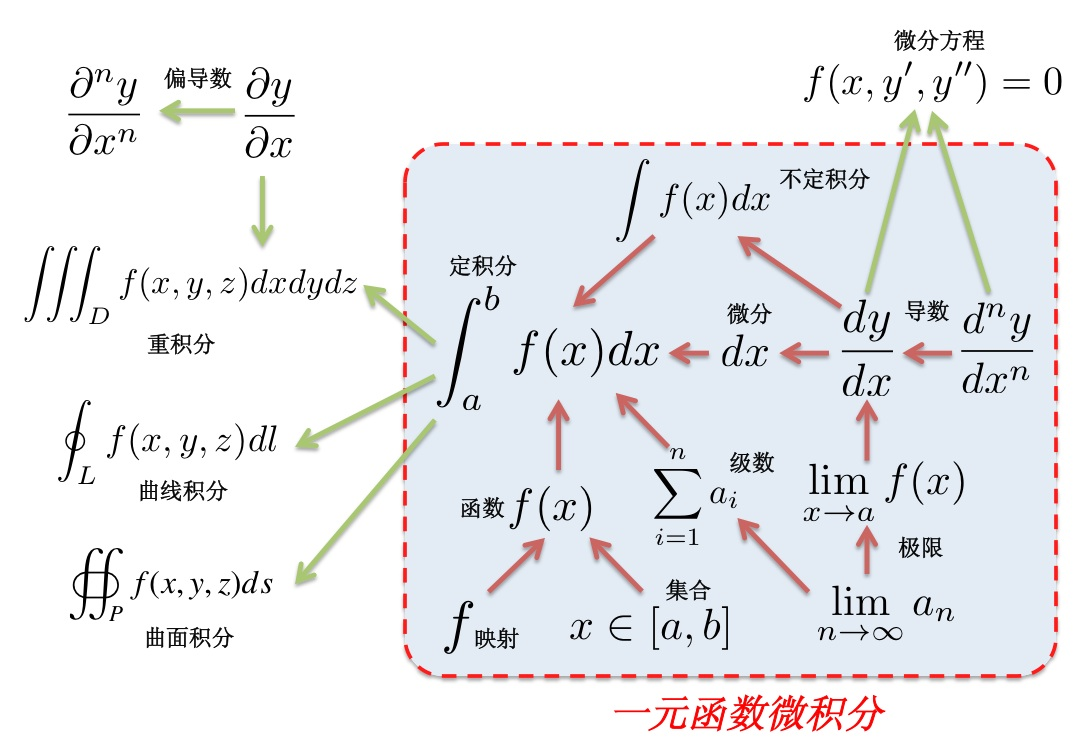
\includegraphics{./images/ch1/AM_architecture.jpg}}
	\ps{上课前画好}
\end{center}

\subsection{怎么学}
	
\begin{itemize}
	\item {\bf 参考资料}
  	\begin{enumerate}
		\item {\bf 课程配套辅导}
	  	\begin{itemize}
	    	\item {李建平 等,高等数学典型例题与解法(上、下),国防科技大学出版社,2009,长沙} 
	  	\end{itemize}
  		\item {\bf 参考书} 
  		\begin{itemize}
	    	\item {\b 同济大学数学系,高等数学(第六版,上、下),高等教育出版社,2006,北京} 
	    	\item 菲赫金哥尔茨,微积分学教程(第一至三卷),第8版,高等教育出版社,2006,北京 
	    	\item James Stewart, Calculus(5th eds.)(影印版,上、下册),高等教育出版社,2004,北京
	    	\item 任何有关教学内容和{\b 数学历史}的书籍
  		\end{itemize}
	\end{enumerate}
	  \item {\bf 学习方法}
	\begin{itemize}
	  		\item {\bf 听课}\dotfill {\bb 30}
		\begin{itemize}
	  		  \item 典型问题、典型方法
	    	  \item 师傅领进门,修行在个人
	 	\end{itemize}
	  		\item {\bf 练习}\dotfill {\bb 50}
	 	\begin{itemize}
	    		\item 熟能生巧!
	    		\item 记忆!琢磨!
	  	\end{itemize}
	  		\item {\bf 思考}\dotfill {\bb 20}
	  	\begin{itemize}
	    		\item 总结!
	    		\item 质疑!
	  	\end{itemize}
	\end{itemize}
\end{itemize}

\section{几点要求}
\begin{itemize}
	\item {\bf 课堂:安静!安静!!安静!!!}
	
	{\bf - No to}
	  \begin{itemize}
	    \item Chatting
	    \item zZZ\ldots
	    \item anything noisy
	    \item \ldots
	  \end{itemize}
	{\bf - Yes to}
  \begin{itemize}
    \item listen to me
    \item discuss {\bf with me}
    \item do sth. you like {\bf quietly}
    \item zzz\ldots
    \item leave/enter the classroom {\bf quietly}
    \item \ldots
  \end{itemize}
  \item {\bf 作业}
  \begin{itemize}
    \item 正确、规范、工整
    \item no copy !!!!
    \item 订正每一个错误!
  \end{itemize}
	\item {\bf 答疑}
	  \begin{itemize}
	    \item 有问必答
	    \item 除了问考试、问隐私
	  \end{itemize}
% 	  \item {\bf 从善如流}
\end{itemize}

\chapter{映射与函数}

{\bf 关键词:}集合、集合论、映射、函数、曲线及其表示

\section{集合与映射}

\subsection{集合}

{\it Cantor,1874:}\ps{对于集合,“我们只需描述它,而不必给出精确的定义”}
所谓{\b 集合},是指把一些个体({\b 元素}) 放在一起考虑时它们形成的整体。
\begin{itemize}
  \item 关系符号:$\subset, \in, =, \subseteq, \neq$
  \item 运算符号:$\cap,\cup, \setminus, \bar{A}, \times, +, - $
\end{itemize}
	
{\bf 常见(用)的集合:}
$\mathbb{N}\subset\mathbb{Z}\subset\mathbb{Q}\subset\mathbb{R}\subset\mathbb{C}$
\ps{本书约定,自然数集包含数$0$}
	
{\bf 注:}通过集合的笛卡尔乘积{\b “$\times$”} 可以定义更{\bf “高维”}的集合,例如:\\
	\centerline{$\mathbb{R}^2=\mathbb{R}\times\mathbb{R}$}

\subsection{区间和邻域}

{\bf 例:}$(a,b)=\{x|a<x<b\}=\{x\in\mathbb{R}|a<x<b\},a,b\in\mathbb{R}$

{\bf 例:}$\mathbb{R}=(+\infty,-\infty)$

{\bf 注意:}$\pm\infty$都不是一个具体的数,因此不能写
$$x=+\infty,\quad x=-\infty$$
而只有
$$x\to+\infty,\quad x\to\infty$$

{\bf 邻域:}“与$a$邻近,距离不超过$\delta$”
$$U(a,\delta)=(a-\delta,a+\delta)=\{x||x-a|<\delta\}$$

{\bf 例:}
$$(a,b)=\left(\df{a+b}2,\df{b-a}2\right)$$

{\bf 去心邻域}
$$U_0(a,\delta)=(a-\delta,a+\delta)-\{a\}=\{x|0<|x-a|<\delta\}$$

{\bf 无穷邻域}
$$\{x||x|>M\},\;M>0$$

{\bf 问:}可以写成$U(\infty,M)$吗?

{\bf 注:}类似地,可以有所谓的半邻域,左(右)邻域

\begin{shaded}

{\bf 集合论、Russell Paradox与公理系统}

	{\it Cantor,1874:}朴素集合论的诞生。	

	{\it Poincare,1900,国际数学家大会:} 
		 {“\ldots 借助集合论概念,我们可以建造整个数学大厦\ldots  今天,我们可以说绝对的严格性已经达到了\ldots”}
	
	{\it Russell, 1901:}只给不给自己理发的人理发的理发师该不该给自己理发?
	
	“由所有不包含集合自身的集合所构成的集合”,记为$S$。不论$S$是不是自身的元素,按照$S$的定义都会有矛盾。
	
	设$x\in A$表示:$A$给$x$理发, 定义
	$$A=\{x|x\notin x\},$$ 
	
	问:$A\in A$还是$A\notin A$? 
	
% 	\ba{罗素悖论导致了第三次“数学危机”的出现!}
	{{\bf {第三次“数学危机”}}(Frege,1901,《算术基础》)}
		“在工作结束之后发现那大厦的基础已经动摇,对于一个科学工作者来说,没有比这更不幸的了”
		
	\begin{itemize}
	  \item {{\bf 无限抽象原则}(Cantor,Frege):} 任意给定某个条件就可以确定一个集合。(每个概念的外延可以确定一个集合)
	  \item {\bf 观点:}不加限制地使用无限抽象原则将导致罗素悖论
	  \item {{\bf 有限抽象原则}(限制公理):} 如果已知一个集合和一个给定的条件,
	  则该集合中所有满足条件的元素{\it 可以}构成一个集合。
	  \item {\bf ZFS(Zermelo-Fraenkel-Skolem)公理化集合系统}
	  
	  {\bf 命题:}在ZFS中,无法定义包含所有集合的集合。
	
	{\bf 证明:}反证法。设$A$是一个这样的集合。定义
	$$B=\{x\in A|x\notin x\}$$
	若
	$B\in A$,则必有$B\in B$或$B\notin B$。而若$B\in B$,可推出$B\notin B$;同理,
	由$B\notin B$,也可推出$B\in B$。从而$B\notin A$,推出矛盾。这说明$B$的定义存在问题,故知假设错误。

	\item {\bf 公理(Axiom):}无须证明即为正确的命题。
	\begin{itemize}
	  \item {\bf Engles:}数学上的所谓公理,是数学需要用作自己出发点的少数思想上的规定 
	  \item {\bf ZFS系统:}公理就是一些关于逻辑符号{“$\in$”}和{字母}的组合使用方法的约定
	  \item {\bf 公理化方法}是构建现代数学理论体系的基石
	\end{itemize}
	\item {\bf {数学等于永恒的真理吗?}}
	\end{itemize}
\end{shaded}
	
\subsection{实数集的性质}
	\begin{enumerate} 
	  \item {\bf 有序性}($\mathbb{R}^2$、$\mathbb{C}$不具备有序性) 
	  \ps{$\mathbb{R}$是全序的,而$\mathbb{R}^2$、$\mathbb{C}$在一定的度量下
	  是半序的}
	  \item {\bf 完备性(连续性): }实数集与数轴上的点之间存在一一对应
	  
	  {\bf{连续性公理(确界原理):}}非空有{上界}的实数集必有{上确界} (最小的上界)
	\end{enumerate}
	
	{\bf 注:}有理数集不满足连续性公理。
	\ps{有理数集的有限次四则运算仍是有理数}
	
	{\bf 例:$e=\mathrm{sup}\left\{\left(1+\frac
	1n\right)^n\right|n\in\mathbb{N}\}\notin\mathbb{Q}$}
	\begin{center}
		\resizebox{!}{5cm}{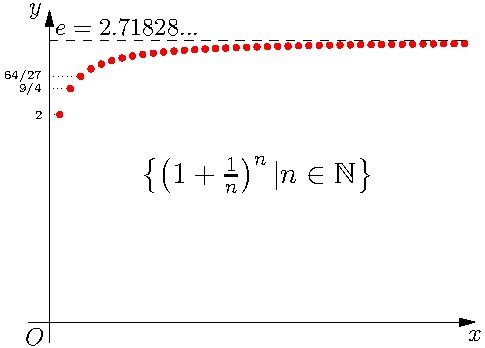
\includegraphics{./images/ch1/e-notin-N.pdf}}
% 		\resizebox{!}{4.8cm}{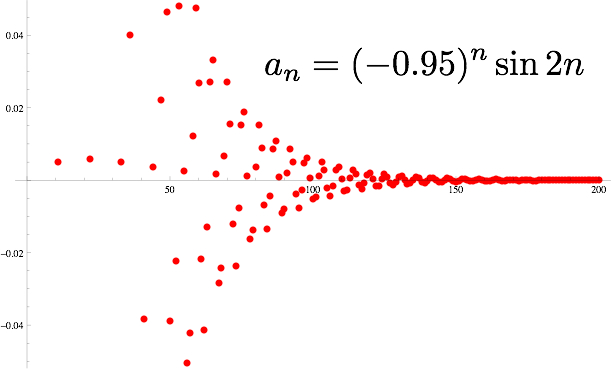
\includegraphics{./images/ch2/sin2nn.jpg}}
% 		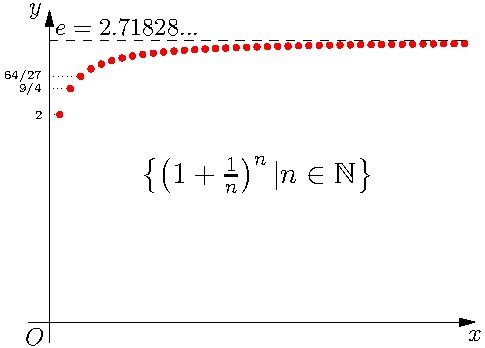
\includegraphics[width=6cm]{./images/ch1/e-notin-N}
	\end{center}
	$$\left(1+\frac11\right)^1<\left(1+\frac12\right)^2<\left(1+\frac13\right)^3<\ldots
	\left(1+\frac1n\right)^n<\ldots<e$$
	
	{\bf 思考:}上确界和最大值有什么异同?如何确定一个集合的上确界?

\subsection{映射}

{\bf 教材P7:}事物之间“一对一”或“多对一”的依赖关系\ps{映射结果必须是无歧义的!}

$$f:A\to B$$
或
$$y=f(x),\;x\in A,y\in B$$

{\bf 三要素:}定义域、值域、对应关系,任何一项不明确都不足以确定一个函数
\ps{有时候只有定义域和对应关系亦可,前提是默认假设映射为满射}

{{\bf 例:}以下函数中哪些是完全相同的?}
		$$x,\quad |x|,\quad e^{\ln x},\quad \ln(e^x),\quad \sqrt{x^2},\quad
		\frac{x^2-4}{x-2}-2,$$
		$$\sin(\arcsin x),\quad \arcsin(\sin x), \quad \tan(\arctan x)$$

{\bf 相关概念:}单射、满射、一一映射(双射)

\begin{shaded}
	{\bf 一一映射与无穷集合}
	
{\bf 问题:}如何比较两个集合中元素的个数?
\begin{itemize}
  \setlength{\itemindent}{1cm}
  \item 自然数与正偶数“一样多”?({$\surd$})
  \item 自然数与整数“一样多”?({$\surd$})
  \item 自然数与有理数“一样多”?({$\surd$})
  \item 区间$(a,b)$中的实数与$\mathbb{R}$中“一样多”?({$\surd$})
  \item 自然数与实数“一样多”?({$\times$})
\end{itemize}
	
{\bf 无穷集合:}可以和自身的某个子集建立起一一映射的集合
\end{shaded}	

	
\section{函数}
	
	\begin{shaded}
		{\bf 关于函数}
		\begin{itemize}
  		  \setlength{\itemindent}{1cm}
		  \item 微积分是关于运动和变化的数学;
		  \item 函数是对运动(例如:曲线、曲面、波以及各种变化)变化过程中各种量与量的依赖关系的抽象描述;
		  \item 函数刻画了运动变化中的量之间的相互依存关系({\bf 注:}与“依存”对应的关系叫做“独立”)
		\end{itemize}
		
		{\bf 常量和变量}
		\begin{itemize}
  		  \setlength{\itemindent}{1cm}
		  \item {\bf 常量和变量是相对的},在一定条件下可以相互转化
		  \item 变量之间的关系可能是相互依存,也可能是相互独立的
		  \item 为了避免讨论过于复杂,简化问题,我们可能选择只考虑部分参数的变化,而将其他参数视为(或设为)常量,
		  例如:万有引力与两个物体的质量、距离以及引力常数(系数)都有关,为了确定其数量关系,需要事先假定部分的参数
		  值是固定不变的
		\end{itemize}
		
		{\bf 大学数学与中学数学}
		\begin{itemize}
  		  \setlength{\itemindent}{1cm}
		  \item 数学并无严格的“高等”和“初等”之分,只是存在众多的分支和领域
		  (例如:代数、几何、分析、图论,几何又分为平面几何、立体几何、解析几何等),
		  不同分支或领域的直观性和难度各有不同
		  \item 对于函数,中学阶段更注重在对应关系“确定”的情况下,寻找其数学描述或利用给定的值进行计算
		  \item 大学阶段,从微积分开始,更着重对函数的整体特性,以及不同函数间的转换、类比和关于其整体特征的计算与分析
		\end{itemize}
		
		 {\bf James Stewart, Calculus(5th eds.), 2004}
		  \begin{itemize}
  		    \setlength{\itemindent}{1cm}
		    \item {\it Calculus is fundamentally different from the mathematics that
		    you have studied previously}
		    \item {\it Calculus is less static and more {\b dynamic}}
		    \item {\it It is concerned with change and {\b motion}}
		    \item {\it It deals with quantities that {\b approach} other
		    quantities}%\marginpar{note}
		  \end{itemize}
	\end{shaded}

	{\bf (一元)函数:}由实数集到实数集的映射
	$$f:D\to\mathbb{R},\;(D\subset\mathbb{R})$$
	或
	$$y=f(x),\;(x\in D\subset\mathbb{R},y\in\mathbb{R})$$
% 	\begin{itemize}
% 	  \item {\bf 定义域:} $D\subset \mathbb{R}$ ,且$D\ne\phi$ 
% 	  \item {\bf 对应关系:} $f:D\to\mathbb{R}$
% 	\end{itemize} 
	{\bf 函数图像}
	$$G_f=\{(x,f(x))|x\in D_f\}$$
	
	\begin{shaded}
		{\bf 多元函数:} 
		$$f:D\to\mathbb{R},\quad D\in\mathbb{R}^n$$
		
		{\bf 向量值函数:}
		$$f:D\to\mathbb{R}^,\quad, D\in\mathbb{R}$$
		
		{\bf 思考:}二元函数和三维的向量值函数对应的几何对象分别是什么?
		
		{\bf 思考:}平面曲线与一元函数具有一一对应关系吗?空间曲面和二元函数呢? (No)	
	\end{shaded}	
		\begin{center}
			\resizebox{!}{4.2cm}{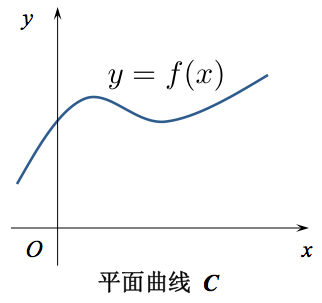
\includegraphics{./images/ch1/C_fx.jpg}}\quad	
			\resizebox{!}{4.5cm}{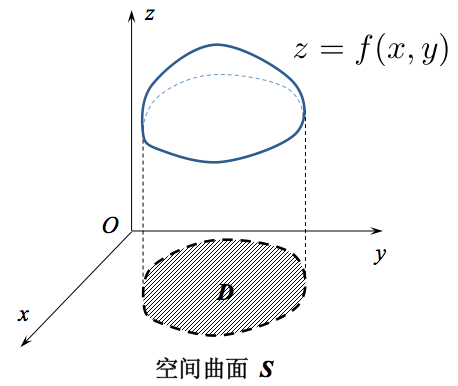
\includegraphics{./images/ch1/S_fxy.jpg}}
		\end{center}
	
\subsection{函数的运算与简单性质}

{\bf 运算:}四则运算、复合运算、逆运算	
	
\begin{shaded}
{\bf 常用数学符号}
	\begin{itemize}
	  \item {$\bm{\forall}$} \quad 任意 (for all)
	  \item {$\bm{\exists}$} \quad 存在 (exist)
	  \item {$\bm{\Rightarrow}$} \quad 推出 (deduce, imply)
	  \item {$\bm{\Leftrightarrow}$} \quad 等价 (equivalent, if and only if)
	  \item {$\bm{\to}$} \quad 趋于 (approach)
	\end{itemize}
\end{shaded}

\subsubsection{【有界性】}			

{{\bf 定义:}}
	设$I\subset\mathbb{R}$,$f(x)$在$I$上有定义,若集合
	$$\{f(x)|x\in I\}$$
	有界,则称{\bf $f(x)$在$I$上有界}或{\bf $f(x)$是$I$上的有界函数}
		
	{\bf 注:}函数的有界性等价于其值域的有界性

	{{\bf 例:}指出如下函数的有界性}
	
		\quad(1)\;$y=\arctan x$,\hspace{2em} (2)\;$y=e^x$,\hspace{2em}
		(3)\;$y=x\sin x$
		
\begin{shaded}
	{\bf “反面定义”(否命题)的写法*}
	\begin{enumerate}
	  \item {“任意”和“存在”互换}
	  \item {“$\geq(\leq)$”和“$<(>)$”互换}
	\end{enumerate}
	
	【提示】:参考De Morgen律,任何命题的成立都是与一定范围有关的
	
	{\bf 定义'}(无界性)
		设函数$f:D\to\mathbb{R}$,若对$\forall M$,$\exists x_M\in D$,使得
		$f(x_M)>M$,则称{\bf $f(x)$无上界}。

\end{shaded}		

\subsubsection{【单调性】}

{{\bf 定义:}}设$f:I\to\mathbb{R}$,若$\forall x_1,x_2\in I$
$$x_1<x_2\Rightarrow f(x_1)\leq f(x_2)$$
则称{\bf $f(x)$在$I$上单调递增}(若不等式中的等号总是无法成立,则称其为严格单调递增)
	
{{\bf 例:}讨论如下函数的单调性}

	\quad(1)\;$y=x\mathrm{sgn}(x)$\hspace{3cm}(2)\;$y=x+\sin x$

{\bf 注:}严格单调的函数一定存在反函数。反之呢?\ps{要说明一个命题不成立,只需举出反例即可}

\subsubsection{【奇偶性】}

{{\bf 定义:}}
	设函数$f:\mathbb{R}\to\mathbb{R}$,
	{\bb 称$f(x)$为偶函数},是指: 对$\forall x\in\mathbb{R}$,有
	$$f(-x)=f(x)$$

{{\bf 例:}试给出如下性质的数学定义}
\begin{enumerate}[(1)]
  \setlength{\itemindent}{1cm}
  \item 函数$y=f(x)$的图像关于$x=a$对称
  \item 函数$y=f(x)$的图像关于点$(x_0,y_0)$对称
\end{enumerate}

{{\bf 思考:}$f(x)=g(a-x),\;(x\in\mathbb{R})$有什么几何意义?}

【提示】:$\sin(x)=\cos(\pi/2-x)$

\subsubsection{【周期性】}

{{\bf 定义:}}
设函数$f:\mathbb{R}\to\mathbb{R}$,
称{\bb $f(x)$为周期函数},是指: $\exists T>0$,
使对$\forall x\in\mathbb{R}$,有
$$f(x+T)=f(x).$$
 满足以上性质的最小正数$T$称为$f(x)$的{\bb 最小正周期}
		 
{\bf 注:}若$T$为$f(x)$的一个周期,$n\in\mathbb{Z}$,则$\forall x\in\mathbb{R}$
$$f(x+nT)=f(x)$$

\subsection{常用函数}

\subsubsection{\bf 【符号函数】}

  $$\bm{\mathrm{sgn}}\,x =\left\{
	\begin{array}{rl}
	-1,\;&x<0 \\
	0,\;&x=0 \\
	1,\;&x>0
	\end{array}
  \right.$$
  {\bf 注:}$|x|=x \cdot\mathrm{sgn} x$
	

 \subsubsection{\bf 【取整函数】}

  $$y=\left[ \,x\, \right]$$
  $[\,x\,]$表示小于等于$x$的最大整数

	
{\bf 注:}有时候还有所谓的上取整和下取整函数

{{\bf 例:}给出以下曲线的方程}

\begin{center}
	\resizebox{!}{2.5cm}{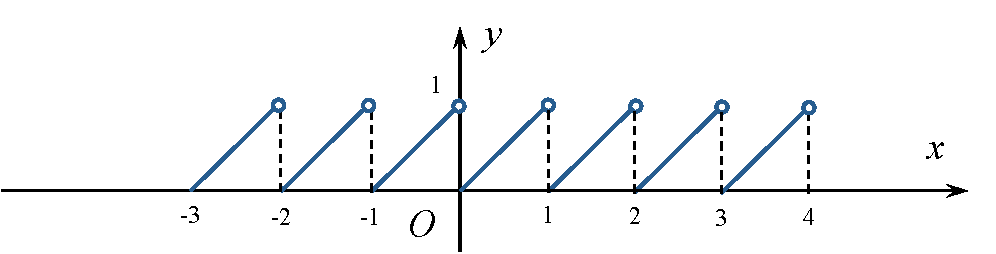
\includegraphics{./images/ch1/f1.pdf}}\quad $x-[x]$\\

	\resizebox{!}{2.5cm}{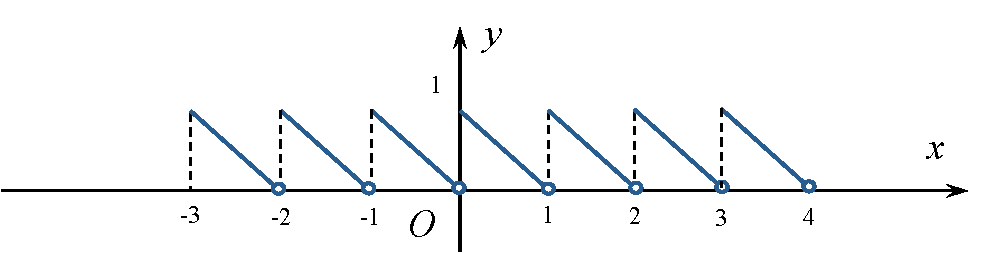
\includegraphics{./images/ch1/f2.pdf}}\quad $[x]-x+1$\\

	\resizebox{!}{2.5cm}{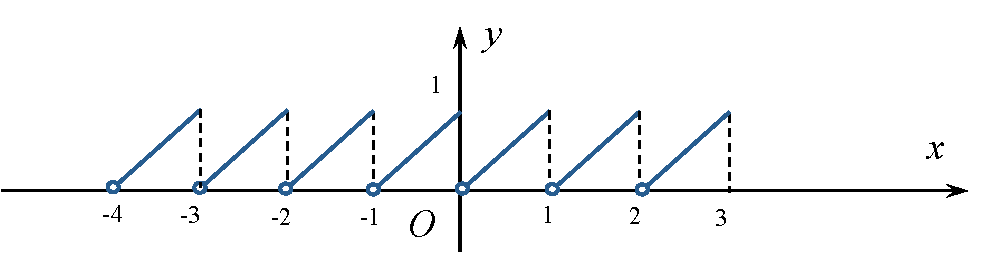
\includegraphics{./images/ch1/f3.pdf}}\quad $[-x]+x-1$
\end{center}
	
{\bf 例:}$(-1)^{[x]}$的图像?方波!

\subsubsection{\bf 【Dirichlet函数】}
  $$\bm{D}(x) =\left\{
  \begin{array}{ll}
  	1,\;& x\in\mathbb{Q} \\
  	0,\;& x\notin\mathbb{Q}
  \end{array}
  \right.$$
  \begin{itemize}
    \item $D(x)$在实数轴上处处无极限
	\item $D(x)$在实数轴上处处不连续
	\item {\b 仅在一点连续的函数:}$xD(x)$
  \end{itemize}

\subsubsection{\bf 【Riemann函数】*:} 

$(x\in[0,1])$
  $$\bm{R}(x) =\left\{
	\begin{array}{ll}
	1,\;&x=0\\
	\displaystyle\frac 1q,\;&x=\displaystyle\frac pq,\,p,q\mbox{互素}\\
	0,\;&x\notin\mathbb{Q}
	\end{array}
  \right. $$
  \begin{itemize}
    \item 对任意$x_0\in[0,1]$, $\lim\limits_{x\to x_0}R(x)=0$
    \vspace{1ex}
    \item $R(x)$在{\b 无理数点连续, 有理数点不连续}
  \end{itemize}

\subsubsection{【初等函数】}

\begin{enumerate}
  \item {\bf 幂函数:} $y=x^a,\; (a\in\mathbb{R})$\ps{只有整数次幂的函数可以手工计算!!!}
  \item {\bf 指数函数:} $y=a^x,\; (a>0,a\ne 1)$
  \begin{itemize}
    \item {\b $y=e^x$}
  \end{itemize}
  \item {\bf 对数函数:} $y=\log_ax,\; (a>0,a\ne 1)$
  \begin{itemize}
    \item {\b$y=\ln x$}
  \end{itemize}
  \item {\bf 三角函数:} $\sin x, \,\cos x,\, \tan x, \,\cot
  x,\, \sec x,\, \csc x$
  \item {\bf 反三角函数:} $\arcsin x, \,\arccos x, \arctan x,
  \ldots$
\end{enumerate}
{\bf{要求:}} 熟练掌握初等函数的定义、性质和相互推导的公式


\subsubsection{【($n$)次多项式(函数)】}

  $$P_n(x)=\sum_{i=0}^na_ix^i,
  \;(a_i\in\mathbb{R},i=1,2,\ldots,n)$$
  \begin{itemize}
    \item { $n$次多项式方程$P_n(x)=0$在$\mathbb{R}$上最多有$n$个根 (包含重根) ,在
    $\mathbb{C}$上有且仅有$n$个根(包含重根)}
    \item { 设$x_i\in\mathbb{C}(i=1,2,\ldots,n)$为$P_n(x)=0$的全部根 ,则
    $$P_n(x)=a_n\prod_{i=1}^n(x-x_i)$$}
    \item { 已知$P_n(x)$在$n+1$个点处的值, 可以唯一确定$P_n(x)$}
  \end{itemize}

\subsubsection{【有理函数】}

$$f(x)=\frac{P(x)}{Q(x)}, \quad\mbox{其中}P(x),Q(x)\mbox{均为多项式函数}$$
  
{\bf 注:}任意有理函数总可以化为一个多项式函数和一个真分式(分子的次数比分母低的有理函数)
的和
	  
{{\bf 例:}用多项式除法化简以下函数}
$$\frac{5x^3+3x^2+1}{x+1}$$

\subsubsection{【双曲函数】}

{\small $$\sinh x =\df{e^x-e^{-x}}{2}, \quad
\cosh x =\df{e^x+e^{-x}}{2}, \quad\tanh x=\df{\sinh
x}{\cosh x}, \ldots$$}

\section{曲线的参数方程和极坐标方程}

{\bf 问题:}$y=f(x)$能否表示平面上的所有曲线?
	
{\bf 或者:}怎样才能更好地表示平面上的曲线?\ps{例如:$x^2+y^2=1,xy=1,x=y^2,\ldots$}

\begin{shaded}
	\begin{center}
		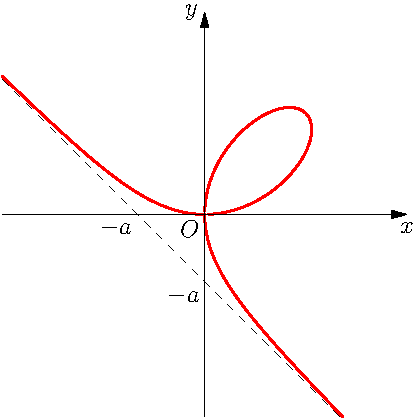
\includegraphics[width=5.5cm]{./images/ch1/dicartesCurve.pdf}

		{\bf Descartes叶形线}
	\end{center}
	\bigskip
	\begin{itemize}
	  \item {\bf 参数方程:}
	  	$$\left\{\begin{array}{l}
	  		x=\df{3at}{1+t^3},\\[1em] y=\df{3at^2}{1+t^3}
	  	\end{array}\right.\;(t\in\mathbb{R})$$
	  	\vspace{-1em}
	  \item {\bf 隐函数方程:}
	  	$$x^3+y^3-3axy=0$$
	\end{itemize}
\end{shaded}

{\bf 例:}求过平面上两点$P_i(x_i,y_i)\,(i=1,2)$的直线方程
		  
$$k=\df{y_2-y_1}{x_2-x_1}=\df{y_2-y_1}{x_2-x_1}$$
由此可给出直线的平面直角方程。若参数化
$$\df{y_2-y_1}{y_2-y_1}=\df{x_2-x_1}{x_2-x_1}=t$$
则有
$$y=ty_2+(1-t)y_1,\quad x=tx_2+(1-t)x_1,\quad (t\in\mathbb{R})$$
		  
{\bf 注:}
\begin{itemize}
  \setlength{\itemindent}{1cm}
  \item 参数方程必须标明参数的取值范围!!!
  \item {利用参数方程可以表示平面上的任意曲线}
  \item {任意曲线的参数方程均不唯一}
\end{itemize}

\subsubsection{【极坐标】}

$$(x,y)\;\to\;(\rho\cos\theta,\rho\sin\theta)\quad
(\rho>0,\theta\in\mathbb{R})$$
	
{{\bf 例:}求以下曲线的极坐标方程\hfill P38-例9}
		
\begin{enumerate}[(1)]
  \setlength{\itemindent}{1cm}
  \item $y=kx,(k\in\mathbb{R})$
  \item $x+y=1$
  \item $x^2+y^2=R^2,\,(R>0)$
  \item $(x^2+y^2)^2=2a^2xy$
\end{enumerate}
	
{\bf 思考:}将极坐标方程化为平面直角方程应注意些什么?

\newpage

\section*{课后作业}
	
\begin{itemize}
  \item 习题1.1:4(2),10
  \item 给出P9例6中二维球极投影映射中:
  
  (1)$Q$的极坐标与$P$的横坐标的对应关系;
  
  (2)$Q$的坐标与$P$的坐标的对应关系;
  
  (3)描述如何将一个单位球面映射为一个二维平面,给出相应的坐标对应关系。
  \item 习题1.2:8,12,13,21
  \item 给出P23例14中的三角波的函数表达式
  \item 习题1.3:5
\end{itemize}

{\bf 【课堂练习与思考题】}

\begin{itemize}
  \item 习题1.1:(C)应用题
  \item 习题1.2:3,17
  \item 习题1.3:6
  \item 阅读:李开复,《给未来的你》
\end{itemize}

\newpage

\section*{参考解答}

1. 习题1.1:10,证明:
$$\df{a_1+a_2+\cdots+a_n}n\geq\sqrt[n]{a_1a_2\cdots a_n},$$
其中$a_i(i=1,2,\ldots,n)$均为非负实数。

证法一:易证$n=2$时不等式成立。假设对$n=2^k(k\in\mathbb{Z}_+)$不等式成立,则
当$n=2^{k+1}$时,
\begin{eqnarray*}
	a_1+a_2+\cdots+a_{2^{k+1}}&\leq&2^k\sqrt[2^k]{a_1a_2\cdots a_{2^k}}
	+2^k\sqrt[2^k]{a_{2^k+1}+a_{2^k+2}+\cdots+a_{2^{k+1}}}\\
	&\geq&2\cdot 2^k\sqrt{\sqrt[2^k]{a_1a_2\cdots a_{2^k}}\cdot
	\sqrt[2^k]{a_{2^k+1}+a_{2^k+2}+\cdots+a_{2^{k+1}}}}\\
	&=&2^{k+1}\sqrt[2^{k+1}]{a_1a_2\cdots a_{2^{k+1}}}
\end{eqnarray*}
由数学归纳法,可知当$n$取$2$的整数次幂时,不等式成立。

若$n$不等于$2$
的某个整数次幂,不妨设$2^{k-1}<n<2^k(k\in\mathbb{N})$,于是
\begin{eqnarray*}
	& &a_1+a_2+\cdots+a_n+\left(2^k-n\right)\sqrt[n]{a_1a_2\cdots a_n}\\
	& & \quad\geq 2^k\sqrt[2^k]{a_1a_2\cdots a_n\left(\sqrt[n]{a_1a_2\cdots
	a_n}\right)^{2^k-n}}\\
	& &\quad =2^k\sqrt[n]{a_1a_2\cdots a_n}
\end{eqnarray*}
以上不等式稍加整理即证。

证法二:易证$n=2$时不等式成立。以下假设$n=k$时不等式也成立,即
$$\df{a_1+a_2+\cdots+a_k}{k}\geq\sqrt[k]{a_1a_2\cdots a_k}.$$
当$n=k+1$时,记$t=a_1+a_2+\cdots+a_k$,且不妨设$a_{k+1}=\max\{a_1,a_2,
\cdots,a_{k+1}\}$,即$ka_{k+1}\geq t$,也是
\begin{eqnarray*}
	\left(\df{a_1+a_2+\cdots+a_{k+1}}{k+1}\right)^{k+1}
	&=&\left(\df{t+a_{k+1}}{k+1}\right)^{k+1}
	=\left[\df tk+\df{ka_{k+1}-t}{k(k+1)}\right]^{k+1}\\
	&\geq&C_{k+1}^0\left(\df tk\right)^{k+1}+C_{k+1}^1\left(\df tk\right)^k
	\df{ka_{k+1}-t}{k(k+1)}\\
	&=&\left(\df tk\right)^ka_{k+1}\geq a_1a_2\cdots a_{k+1}
\end{eqnarray*}
即证。
\bigskip

2.给出P9例6中二维球极投影映射中:
  
(1)$Q$的极坐标与$P$的横坐标的对应关系;
  
(2)$Q$的坐标与$P$的坐标的对应关系;
  
(3)描述如何将一个单位球面映射为一个二维平面,给出相应的坐标对应关系。

解:
\begin{center}
	\resizebox{!}{5cm}{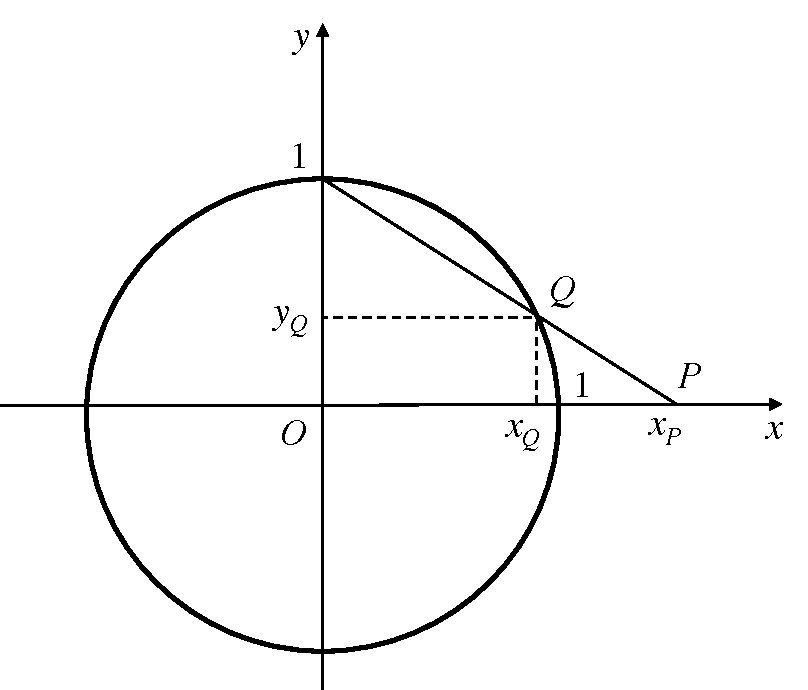
\includegraphics{./images/ch1/answer/sphereline2D.pdf}}\quad
	\resizebox{!}{5cm}{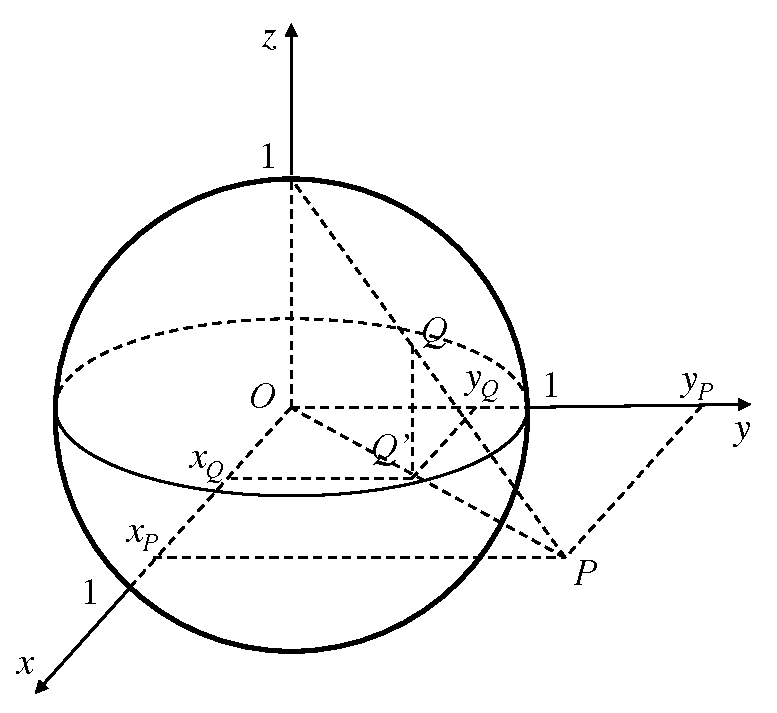
\includegraphics{./images/ch1/answer/sphereline3D.pdf}}
\end{center}
(1)(2) 如左图,设$P,Q$的坐标分别$(x_P,0),(x_Q,y_Q)$,则有
$$
\left\{
\begin{array}{l}
	x^2_Q+y^2_Q=1\\
	\df{x_Q}{x_P}+y_Q=1
\end{array}
\right.
$$
由此可解得
$$y_Q=\df{1-x^2_P}{1+x^2_P},\quad x_Q=\df{2x_P^3}{1+x^2_P}.$$
进而可知$Q$的极坐标为$(1,\theta)$,其中
$$\theta=
\left\{
\begin{array}{ll}
	\arctan\df{1-x^2_P}{2x^3_P},& x_P>0\\
	\pi+\arctan\df{1-x^2_P}{2x^3_P}, & x_P<0
\end{array}
\right.
$$
(3)如右图,设$P,Q$的坐标分别$(x_P,y_P,0),(x_Q,y_Q,z_Q)$,则有
$$
\left\{
\begin{array}{l}
	x^2_Q+y^2_Q+z^2_Q=1\\
	\df{x_Q}{x_P}=\df{y_Q}{y_P}=1-z_Q
\end{array}
\right.
$$
由此可解得
$$
\left\{
\begin{array}{l}
	x_Q=\df{2x_P(x^2_P+y^2_P)}{1+x^2_P+y^2_P}\\
	y_Q=\df{2y_P(x^2_P+y^2_P)}{1+x^2_P+y^2_P}\\
	z_Q=\df{1-x^2_P-y^2_P}{1+x^2_P+y^2_P}
\end{array}
\right.
$$

\bigskip

3.习题1.2:8,题略

\begin{center}
	\resizebox{!}{6cm}{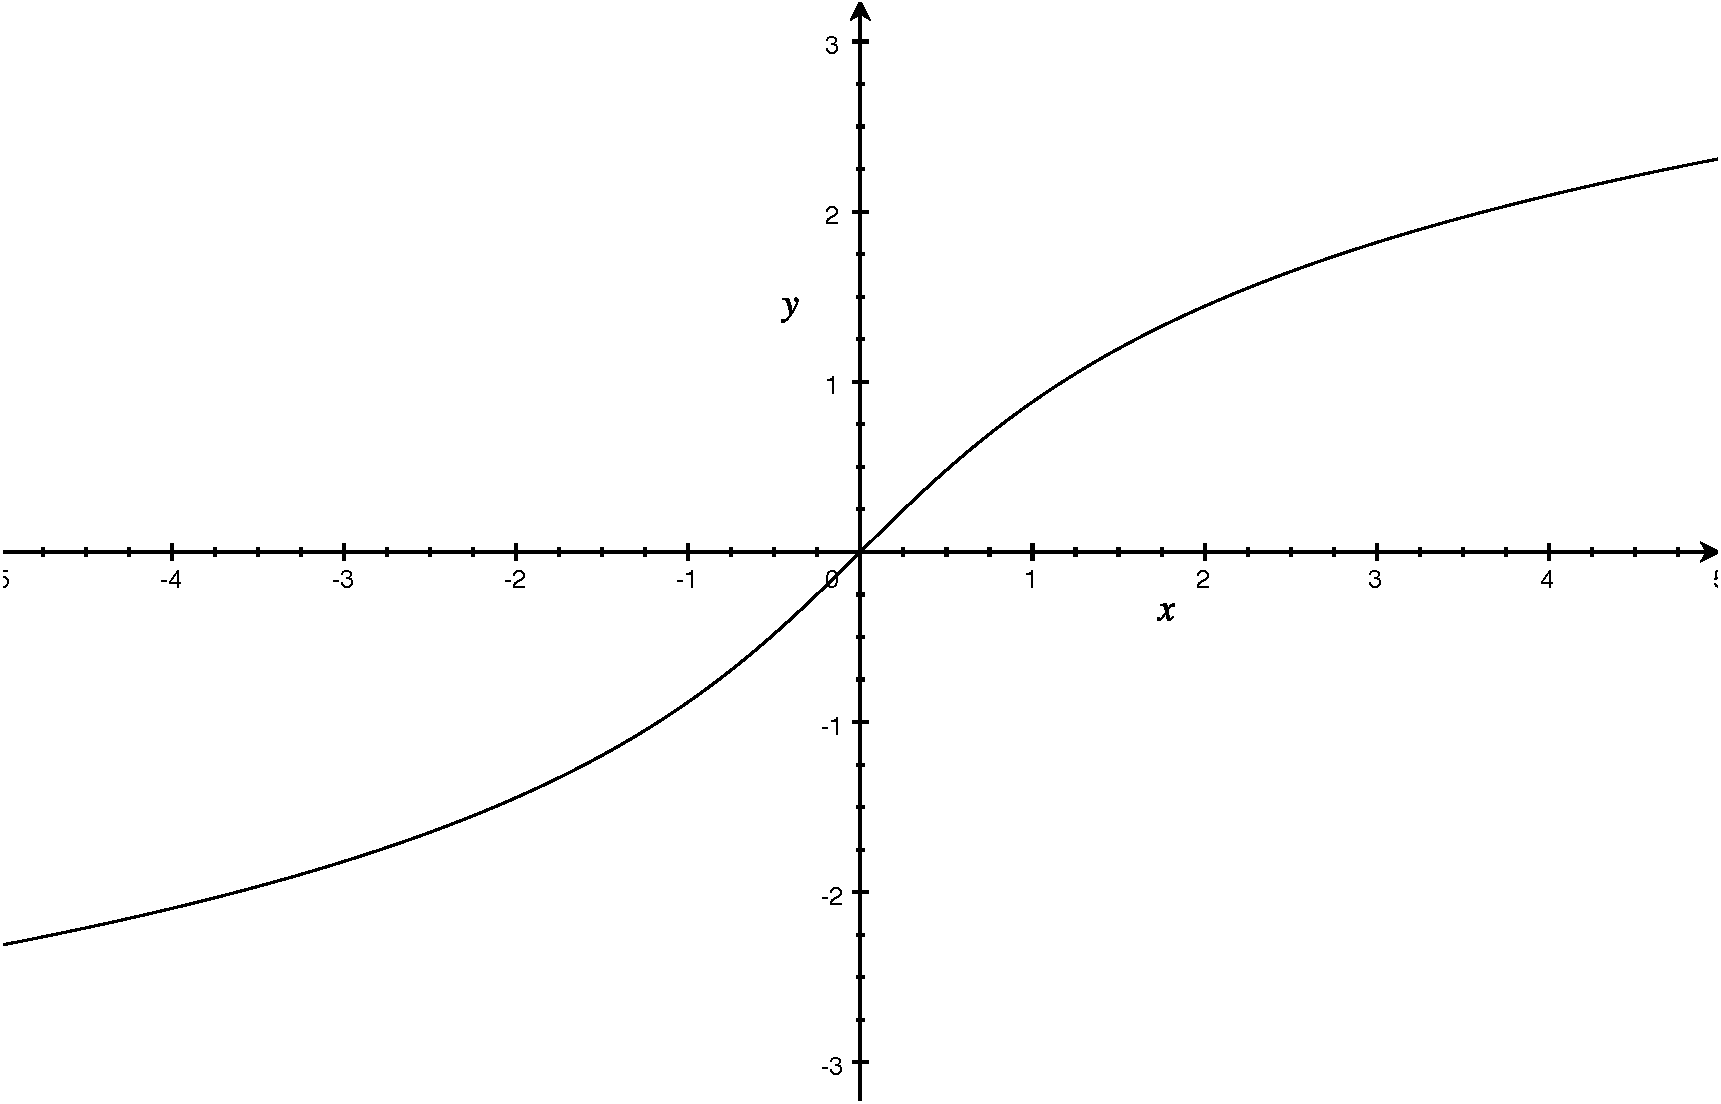
\includegraphics{./images/ch1/answer/lx.pdf}}
	
	$y=\ln(x+\sqrt{1+x^2})$的函数图像
\end{center}

\bigskip

4.习题1.2:17,题略

参考答案:
$$f_c(x)=\df12\left(|f(x)+C|-|f(x)-C|\right)$$

\bigskip

5. 习题5.2:3,证明恒等式

(1)$3\arccos x-\arccos(3x-4x^3)=\pi,\left(|x|\leq\df12\right)$

(2)$2\arctan x+\arcsin\df{2x}{1+x^2}=\pi,(x>1)$

证:(1)注意到
$$\cos(3\arccos x)=4[\cos(\arccos x)]^3-3\cos(\arccos
x)=4x^3-3x=\cos[\pi-\arccos(3x-4x^3)].$$
由此可知
$$3\arccos x=2k\pi-\pi+\arccos(3x-4x^3)\quad(k\in\mathbb{Z}).$$
又当$|x|\leq\df12$时,$|3x-4x^3|\leq 1$,进而
$$\pi+\arccos(3x-4x^3)\in[\pi,2\pi],\quad 3\arccos x\in[\pi,2\pi].$$
从而可知必有
$$3\arccos x=\pi+\arccos(3x-4x^3),$$
即证。

(2)由于
$$\sin(2\arctan x)=\df{2\tan(\arctan x)}{1+\tan^2(\arctan
x)}=\df{2x}{1+x^2}=\sin\left(\pi-\arcsin\df{2x}{1+x^2}\right)$$
从而可知
$$2\arctan x=2k\pi+\pi-\arcsin\df{2x}{1+x^2}\quad(k\in\mathbb{Z}).$$
又当$x>1$时,$2\arctan x\in\left(\df{\pi}2,\pi\right),\df{2x}{1+x^2}\in(0,1)$,进而
$$\pi-\arcsin\df{2x}{1+x^2}\in\left(\df{\pi}2,\pi\right),$$
由此可知必有
$$2\arctan x=\pi-\arcsin\df{2x}{1+x^2},$$
即证。
% 
% \setcounter{chapter}{1}

\chapter{数列极限与数值级数}

\section{数列极限}

\subsection{数列}

{\bf 教材P45:}按一定规律排列的无穷多个(相同或不相同的)数,记作:
$$a_1,a_2,\ldots,a_n,\ldots$$
或者$\{a_n\}$。

$\{a_n\}$的实质是定义在$\mathbb{N}_+$上的函数,即所谓的{\bf 整标函数}\ps{教材上的说法是“可视为”},即
$$a_n:\mathbb{N}_+\to\mathbb{R}$$

{\bf 命题:}一个集合是可数的,当且仅当它可以表示为一个数列。

{\bf 思考:}数列与集合有哪些区别?\ps{1、有序-无序;2、无限-可能有限;3、可重复-不可重复}

{\bf 例:}数列举例

\begin{enumerate}[(1)]
  \setlength{\itemindent}{1cm}
  \item[(1)] $\left\{\df{n+1}n\right\}:\df 21,\df 32,\df43,\df54,\df65,\ldots$
  \item[(2)] $\left\{\df{(-1)^n}n\right\}:-1,\df12,-\df13,\df14,-\df15,\df16,\ldots$
  \item[(3)] $\{n^2\}:1,4,9,16,25,36,\ldots$
  \item[(4)] $\left\{n^{(-1)^n}\right\}:1,2,\df13,4,\df15,6,\ldots$
\end{enumerate}

\subsection{数列的极限}

{\bf 极限:} 一种无限靠近的趋势 
	
\begin{enumerate}
  \setlength{\itemindent}{1cm}
  \item 对于数列而言,无限靠近的趋势意味着什么? 
  \item 如何从数学上严格表达这种趋势? 
\end{enumerate}

{\bf 定义2.1.2} 

对于数列$\{a_n\}$,若存在常数$a$,对于任意给定的正数$\e$,均存在正整数$N$,当$n>N$时,恒有
$$|a_n-a|<\e$$
成立,则称{\bf 数列$\{a_n\}$存在极限(或收敛)},常数$a$称为该数列的极限,记为
$$\lim_{n\to\infty}a_n=a$$
或
$$a_n\to a\;(n\to\infty)$$
若上述常数$a$不存在,则称数列$\{a_n\}$不存在极限(或{\bf 发散})。

\begin{center}
	\resizebox{!}{3cm}{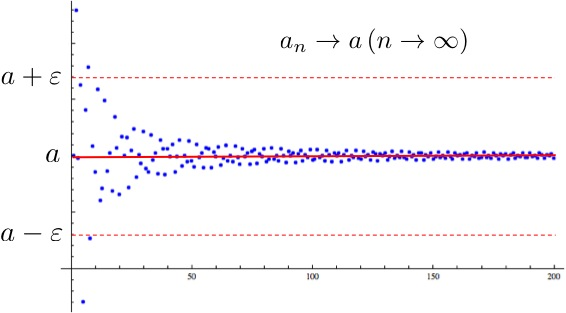
\includegraphics{./images/ch2/lim-en/en1.jpg}}\quad
	\resizebox{!}{3cm}{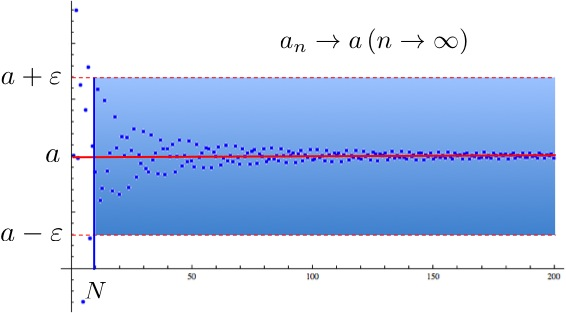
\includegraphics{./images/ch2/lim-en/en2.jpg}}
	
	\resizebox{!}{3cm}{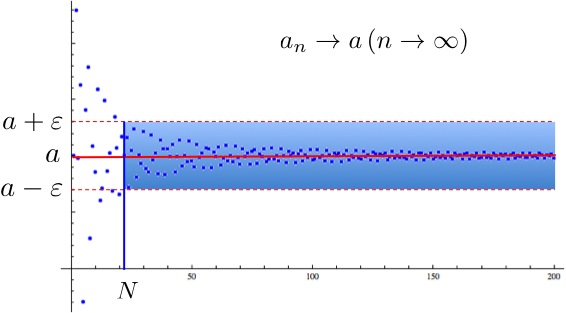
\includegraphics{./images/ch2/lim-en/en3.jpg}}\quad
	\resizebox{!}{3cm}{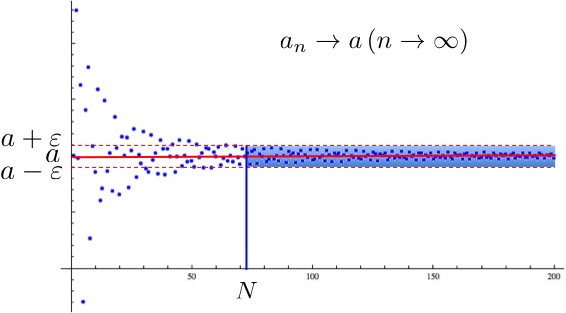
\includegraphics{./images/ch2/lim-en/en4.jpg}}
	
	\resizebox{!}{3cm}{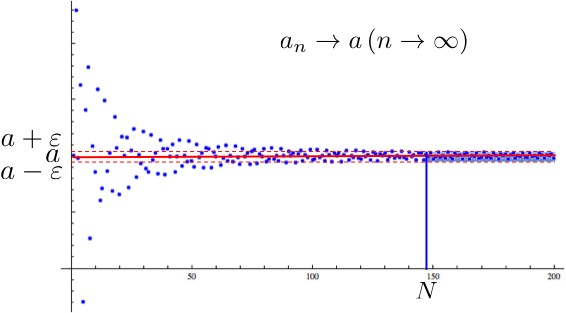
\includegraphics{./images/ch2/lim-en/en5.jpg}}
\end{center}

等价说法:

$$\lim_{n\to\infty}a_n=a\Leftrightarrow
\forall\e>0,\exists N\in\mathbb{Z}_+,\forall n>N,|a_n-a|<\e\eqno{(1)}$$

{\bf 讨论:}以下说法和$(1)$等价的是:

\begin{enumerate}
  \setlength{\itemindent}{1cm}
%   \item[(2)] $\forall\e>0$,$\exists N>0$,$\forall
%   n>N$,$|a_n-a|<\e$ \hfill{$\surd$}\\
%   \hfill(直接写$\exists N$即可)
  \item[(2)] $\forall\e>0$,$\exists N$,$\forall
  n>N$,$|a_n-a|\leq\e$ \hfill{$\surd$} 
  \item[(3)] $\exists N>0$,$\forall\e>0$,$\forall
  n>N$,$|a_n-a|<\e$ \hfill{$\times$} 
  \item[(4)] $\forall\e>0$,仅有有限多个$n$,使得$|a_n-a|\geq\e$
  \hfill{$\surd$} 
  \item[(5)] $\forall\e>0$,总有无穷多个$n$,使得$|a_n-a|<\e$
  \hfill{$\times$} 
  \item[(6)] $\forall\e>0$,要使$|a_n-a|<\e$,只须$n$充分大 \hfill{$\surd$}
  \item[(7)] $\forall\e>0,\exists N\in\mathbb{N}_+,\forall
  n>N,|a_n-a|<2\e$\hfill{$\surd$}
\end{enumerate}

{\bf 注:}

\begin{itemize}
  \setlength{\itemindent}{1cm}
  \item $a$是确定的数 ( {不能是$\pm\infty$}) 
  \item “$\forall\e>0$”应该理解为{“对任意小的$\e>0$”}
  \item $N$由$\{a_n\}$和$\e$共同决定, “存在$N$”可理解为{“存在充分大的$N(\e)$}”; 
   {如果$N$能够满足定义, 任意比$N$大的数都能够满足定义; 通常$\e$取得越小,
  $N$需要取得越大} \ps{$\{a_n\}$的收敛性与其任意多的有限项无关!!}
  \item 给定$C>0$,“$|a_n-a|<\e$” 可替换为{“$|a_n-a|<C\e$”}, 其中$C>0$为常数
\end{itemize}

{\bf 例:}证明:
$$\limn(-1)^n\df1{n^2}=0$$

{\bf 例:}证明:
$$\limn\left(\df n{n+1}\right)^2=1$$

{\bf 例:}证明:若$\limn a_n=a$,则$\limn|a_n|=|a|$

{\bf 例:}证明:若$|q|<1$,则$\{q^n\}$收敛。

{\bf 思考:}已知$|q|>1$时,$\{q^n\}$发散,请问该如何证明?

{\bf 注:}利用有界性,也可以证明发散。

\begin{shaded}
	{\bf 【极限定义的反面说法】}
	
	$$\limn a_n\neq a\Leftrightarrow\exists\e_0>0,\forall N>0,\exists
		n_0>N,|a_{n_0}-a|\geq\e_0$$
	
	{\bf 例:}证明:$\limn\df 1n\neq 1$
	
	{\bf P51,例5:}证明$\{(-1)^n\}$发散。 
	
	{\bf 注:}对比教材上的证明方法与用反面说法证明的区别。
	
	{\bf 思考:}数列发散可能有哪些不同的情形?(趋向无穷,或振荡)
	
\end{shaded}

\subsection{数列极限的基本性质}

\subsubsection{【唯一性】}

{\bf 定理2.1.1:}数列极限若存在,必唯一。\ps{唯一性的要求决定了当前的极限定义。
“记录重大技术突破的技术发展史其实就是一部人类社会发展的技术选择史”}

\begin{center}
	\resizebox{!}{4cm}{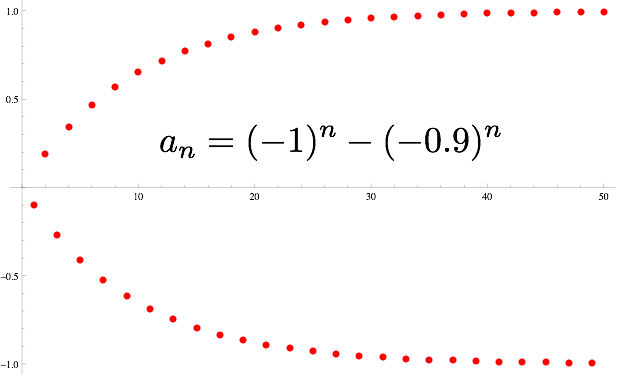
\includegraphics{./images/ch2/1-0.9n.jpg}}
\end{center}

{\bf 典型方法:}若对$\forall\e>0$,有$|a-b|<\e$,则$a=b$

\subsubsection{【有界性】}

{\bf 定理2.1.2:}数列$\{a_n\}$若收敛,则$\{a_n|n\in\mathbb{Z}_+\}$必有界。

\begin{center}
	\resizebox{!}{4cm}{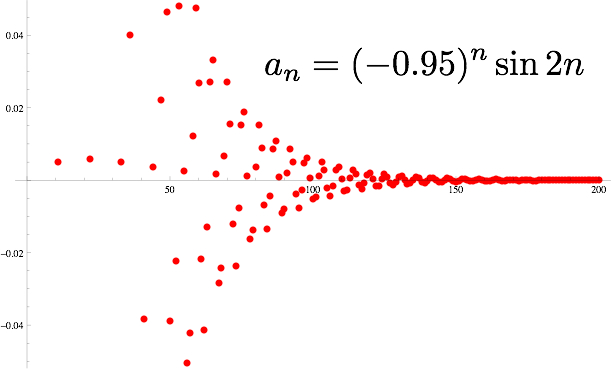
\includegraphics{./images/ch2/sin2nn.jpg}}
\end{center}

{\bf 典型方法:}利用$\e$的特定取值控制无穷的部分,剩余的有限集自然是有界的

{\bf 例:}讨论$\{\sqrt[n]{n!}\}$的敛散性。

{\bf hint:}注意到$\forall a>0$,当$n$充分大时,$n!>a^n$,故$\{\sqrt[n]{n!}\}$无界,
从而发散。

\subsubsection{【保号性】}

{\bf 定理2.1.3:}设$\lim\limits_{n\to\infty}a_n>0$,则$\exists N>0$,
		对$\forall n>N$,$a_n>0$
		
{{\bf 推论:}} 
\begin{enumerate}
  \setlength{\itemindent}{1cm}
  \item 设对$\forall n\in\mathbb{N}$,$a_n\geq
  0$, $\lim\limits_{n\to\infty}a_n=a$, 则$a\geq 0$ 
  \item 设$\lim\limits_{n\to\infty}a_n=a\ne
  0$, 则$\exists N$,当$n>N$时,$|a_n|>|a|/2$ 
  \item
  设$\lim\limits_{n\to\infty}a_n=a$, 且最多有有限个$a_n$小于零, 则$a\geq 0$
\end{enumerate}	

{\bf 注:}保号性的实质,是极限运算保持不等号的方向不变
$$a_n\geq b_n\,(n\in\mathbb{Z}_+)\Rightarrow\limn a_n\geq\limn b_n$$

\section{数列极限的性质与判敛}

\subsection{四则运算的性质}

{\bf 定理2.2.1:}\ps{强调:只对有限次的四则运算有效!!!}
设数列$\{a_n\},\{b_n\}$分别以$a,b(b\neq 0)$为极限,则
数列$\{a_n\pm b_n\},\{a_nb_n\},\left\{\df{a_n}{b_n}\right\}$均收敛,且
\begin{enumerate}
  \setlength{\itemindent}{1cm}
  \item $\limn(a_n\pm b_n)=a\pm b$
  \item $\limn a_nb_n=ab$
  \item $\limn\df{a_n}{b_n}=\df ab$
\end{enumerate}

{\bf 注:}极限运算和四则运算可以交换次序——前提是极限存在,且为有限次四则运算

{\bf 例:}
\begin{eqnarray*}
	1&=&\limn \underbrace{\left(\df 1n+\df 1n+\cdots+\df 1n\right)}_{n}\\
	&=&\underbrace{\limn\df1n+\limn\df1n+\cdots+\limn\df1n}_{n}\\
	&=&n\limn\df1n=0
\end{eqnarray*}
$n$落在了极限符号之外,显然错误!!

{\bf P58-例2:}计算极限
$$\limn\df{2n^6+3n^4-n+10}{n^6+n^4+1}$$

{\bf P58-例1:}设$\limn(a_n+b_n)=1$,$\limn(a_n-b_n)=3$,证明$\{a_n\},\{b_n\}$收敛,并求其值。

{\bf 例:}计算极限
$$\limn\df{\cos^n\theta-\sin^n\theta}{\cos^n\theta+\sin^n\theta}\quad
(0\leq\theta\leq\df{\pi}{2})$$

{\bf 定理2.2.1':}初等函数运算可以和极限运算交换次序。

{\bf 例:}设$a_n>0(n\in\mathbb{N})$,$\limn a_n=a$,证明:
$$\limn\sqrt{a_n}=\sqrt a$$

{\bf hint:} 若$a=0$,对$\e^2$,取$N$即可。

\subsection{子数列的收敛性}

{\bf 子数列:}

$$\{a_{n_k}\}:\,a_{n_1},a_{n_2},\ldots,a_{n_k},\ldots$$

{\bf 注:}$\{n_k\}$本质上是一个正整数构成的数列,
所以子数列可以视为两个数列的复合

{\bf 定理2.2.2:}数列收敛,当且仅当其任意子数列收敛,且极限相同。

即:对任意严格单调递增的正整数数列$\{n_k\}$,
$$\limn a_n=a\Leftrightarrow\lim_{k\to\infty}a_{n_k}=a$$
$\{a_{n_k}\}$收敛于$a$的定义: $\forall \e>0$, $\exists
{K}$, $\forall {k>K}$, 有 $$|a_{{{n_k}}}-a|<\e,$$
 记为\ps{强调$k$变化而不是$n$变化}
$$\lim\limits_{{k\to\infty}}a_{n_k}=a\quad \mbox{或}\quad a_{n_k}\to
a\;{(k\to\infty)}$$


{\bf 推论:}若某个数列存在不收敛的子列,或者存在两个极限不相同的子列,则该数列不收敛。

{\bf 例P60,例4:}证明数列$\left\{n^{(-1)^n}\right\}$发散。

{\bf 定理2.2.3}(拉链定理)数列$\{a_n\}$收敛,当且仅当$\{a_{2n}\}$
和$\{a_{2n-1}\}$收敛于相同的极限。

{\bf 推论:}数列$\{a_n\}$收敛,当且仅当$\{a_{3n}\}$,$\{a_{3n+1}\}$和
$\{a_{3n+2}\}$收敛于相同的极限。

{\bf 注:}更一般性的推广:如果选择的子列能够完全覆盖原数列,或最多不能覆盖原数列中
有限多个数,且这些子列均收敛于相同的极限,则原数列收敛。

\subsection{夹逼(迫敛)定理}

{\bf 定理2.2.4:}设对任意$n\in\mathbb{N}$,$x_n\le a_n\le y_n$,
且$\{x_n\},\{y_n\}$收敛于相同的极限$a$,则$\limn a_n=a$。

\begin{center}
	\resizebox{!}{5cm}{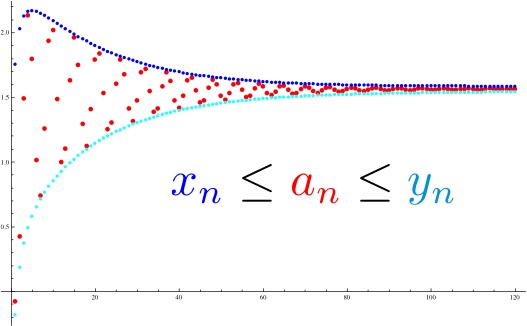
\includegraphics{./images/ch2/xay_n.jpg}}
\end{center}

{\bf P61,例5:}证明$\limn [(n+1)^k-{n}^k]=0$,其中$0<k<1$。

{\bf hint:}$n^k\left[\left(1+\df1n\right)^k-1\right]
<n^k\left(1+\df1n-1\right)=n^{k-1}\to 0\;(n\to\infty)$

{\bf P61,例6:}设$a>0$为常数,证明$\limn \sqrt[n]{a}=1$。

\subsection{单调有界原理}

{\bf 定理2.2.5:}单调有界的数列必收敛。\ps{只要数列从某一项开始单调即可!!!}

{\bf 【重要极限】}(P63-例7)
$$a_n=\left(1+\df{1}{n}\right)^n\to e\quad (n\to\infty)$$

{\bf 注:}需要掌握的重要性质
\begin{itemize}
  \setlength{\itemindent}{1cm}
  \item 数列$\left\{\left(1+\df 1n\right)^n\right\}$严格单调递增有上界
  \item 数列$\left\{\left(1+\df 1n\right)^{n+1}\right\}$严格单调递减有下界
  \item 显然,二者极限相同
\end{itemize}

\subsection{递推数列的判敛}

{\bf 例:}已知$a_1,a_2$为常数,数列$\{a_n\}$满足:
$$a_n=\df 12({a_{n-1}+a_{n-2}})\quad(n>2).$$
证明$\{a_n\}$收敛,并求其极限。

{\bf P65-例9:}设$a_1>0$,$a_{n+1}=\df 12\left(a_n+\df 1{a_n}\right)\,
(n=1,2,\ldots)$,证明$\{a_n\}$收敛,并求其极限。

{\bf 注:}
\begin{itemize}
  \setlength{\itemindent}{1cm}
  \item 递推式两边同时取极限,解方程求得极限的值,是最便利的计算递推数列极限的方法
  \item 若通过以上方法可以求出极限的值,通常只需证明数列单调有界即可
  \item 若该方法无法求得极限的值,则只能利用递推式推导数列通项,进而证明其收敛并计算极限
\end{itemize}

{\bf 例:}计算下列极限
\begin{enumerate}[(1)]
  \setlength{\itemindent}{1cm}
  \item $\limn\df{n^2}{a^n}\quad (a>1)$
  \item $\limn\df{n!}{n^n}$
  \item $\limn\underbrace{\sqrt{c+\sqrt{c+\ldots+\sqrt{c}}}}_{n\mbox{\small
		  个根号}}$
\end{enumerate}

{\bf }若极限存在,可由通项公式反推递推式,然后两边取极限,解方程求得极限值

\begin{shaded}

\subsection{特殊的极限计算方法}

{\bf Stolz定理:}

设数列$\{y_n\}$满足$\limn\df 1{y_n}=0$,且$\{y_n\}$至少从某一项开始保持严格单调递增,
则对任意数列$\{x_n\}$,若$\limn\df{x_n-x_{n-1}}{y_n-y_{n-1}}$存在,则必有
$$\limn\df{x_n}{y_n}=\limn\df{x_n-x_{n-1}}{y_n-y_{n-1}}$$

{\bf 注:}Stolz定理主要用于计算"$\df{\infty}{\infty}$型"的极限

{\bf 推论:}若数列$\{a_n\}$收敛,则
$$\limn\df{a_1+a_2+\ldots+a_n}{n}=\limn a_n$$

{\bf 例:}计算以下极限
\begin{enumerate}[(1)]
  \setlength{\itemindent}{1cm}
  \item $\limn\df{1+\sqrt 2+\sqrt[3]{3}+\ldots+\sqrt[n]{n}}{n}$ 
  \item $\limn\df{1^k+2^k+\ldots+n^k}{n^{k+1}},\quad(k\in\mathbb{N})$ 
  \item $\limn\left(\df{1^k+2^k+\ldots+n^k}{n^{k}}-\df
  n{k+1}\right),\quad(k\in\mathbb{N})$\\
  {\bf 提示:}(3)
  \begin{eqnarray*}
  	\mbox{原式}&=&\limn\df{(k+1)(1^k+2^k+\cdots+n^k)-n^{k+1}}{n^k(k+1)}\\
  	&=&\limn\df{(k+1)(n+1)^k-[(n+1)^{k+1}-n^{k+1}]}{(k+1)[(n+1)^k-n^k]}\\
  	&=&\limn\df{(k+1)[n^k+kn^{k-1}+P_{k-2}^{(1)}(n)]
  	-\left[(n+1)^k+(n+1)^{k-1}n+\cdots+n^k\right]}{(k+1)
  	\left[(n+1)^{k-1}+(n+1)^{k-2}n+\cdots+n^{k-1}\right]}\\
  	&=&\limn\df{(k+1)[n^k+kn^{k-1}+P_{k-2}^{(1)}(n)]-(k+1)n^k
  	-\df{k(k+1)}2n^{k-1}-P_{k-2}^{(2)}(n)}
  	{(k+1)\left[\df{k(k+1)}{2}n^{k-1}+P_{k-2}^{(3)}(n)\right]}\\
  	&=&\df12
  \end{eqnarray*}
\end{enumerate}

\end{shaded}

\section{数值级数}

{\bf 级数(无穷和):}无穷多个数按照一定次序求和
$$\sum\limits_{k=1}^{\infty}a_k
=\lim_{n\to\infty}\left(\sum_{k=1}^na_k\right)$$  
其中$a_k\in\mathbb{R}\,(k\in\mathbb{N})$。

\begin{itemize}
  \item {\bf 部分和(数列):}$S_n=\sum\limits_{k=1}^na_k$
  \item {\bf 级数收敛}$\Leftrightarrow\{S_n\}$收敛
\end{itemize}

{\bf 例:}判断下列级数的收敛性
\begin{enumerate}[(1)]
  \setlength{\itemindent}{1cm}
  \item $\sumn q^n\quad (q>0)$ (\ldots\ldots 几何级数) 
  \item $\sumn\df{1}{n(n+1)}$ 
  \item $\sumn\df 1n$ (\ldots\ldots 调和级数) 
% 		  \item $\sumn\df 1n^2$
  \item $\sumn (-1)^n$
\end{enumerate}

\subsection{收敛级数的性质}

\begin{enumerate}[{\bf 【性质1】}]
  \item {\bf P74-定理2.3.1}(级数收敛的必要条件) 
  $$\sumn a_n\mbox{收敛}\Rightarrow\limn a_n=0$$
  \item $\sumn
  a_n$收敛$\Leftrightarrow\sum\limits_{n=k}^{\infty}a_n$收敛$(k\in\mathbb{N})$
  \ps{讨论收敛性时只需考虑部分和的后一部分,因为数列的收敛性与其前任意项无关}
  \item {\bf P73-例2:}$\{a_n\}$收敛$\Leftrightarrow\sumn(a_{n+1}-a_n)$收敛
  \item {\bf P75-定理2.3.2-3:}线性运算不改变级数的敛散性  
  \item {\bf P75-定理2.3.4:}增加、减少或改变级数中的有限项不影响其敛散性  
  \begin{itemize}
    \item {{增减或改变数列中的有限项不改变其敛散性}} 
  \end{itemize}
  \item {\bf P75-定理2.3.5:}若$\sumn a_n$收敛,不改变求和顺序,
  任意合并其中的项,所得新的级数仍收敛 
  \begin{itemize}
    \item {\bf 推论:}合并收敛级数中的相邻项,所得级数仍收敛 
    \item {{对发散级数,该性质不成立}} 
    \item {{改变求和次序,可能改变级数的收敛和}},例:$\sumn\df{(-1)^n}n$
  \end{itemize}
\end{enumerate}

{\bf 例:}判断以下级数的敛散性;若收敛,求其和

\begin{enumerate}[(1)]
  \setlength{\itemindent}{1cm}
  \item $\sumn\ln\left(1+\df 1n\right)$
  \item
  $\sumn\left[\prod\limits_{k=0}^p(\alpha+n+k)\right]^{-1},\;(p\in\mathbb{N})$
  \item $\sumn\df{x^{2^{n-1}}}{1-x^{2n}}$
  \item $\sumn\df{1}{\sqrt n}$
\end{enumerate}

\section{同号级数的收敛性}

\subsection{同号级数收敛的充要条件}

{\bf 定理2.4.1:}正项级数收敛,当且仅当其部分和数列有界。

{\bf P80,例1:}证明$\sumn\df1{n!}$收敛。

\subsection{比较判别法}

{\bf 定理2.4.2}(比较判别法的不等式形式)若对充分大的$n$,总有$0\leq a_n\leq b_n$,则
\begin{enumerate}
  \setlength{\itemindent}{1cm}
  \item 若$\sumn b_n$收敛,则$\sumn a_n$收敛
  \item 若$\sumn a_n$发散,则$\sumn b_n$发散
\end{enumerate}

{\bf P82-例3:}证明:\ps{p-级数}
\begin{enumerate}[(1)]
  \setlength{\itemindent}{1cm}
  \item[(1)] $p>1$时,$\sumn\df1{n^p}$收敛;
  \item[(2)] $0<p\leq 1$时,$\sumn\df1{n^p}$发散。
\end{enumerate}

{\bf 【hint】:}(2),$p=1$时,显然发散。又因为
$$0<\df 1n<\df 1{n^p},\quad (0<p<1),$$
已知调和级数发散,故p-级数发散;

(1)由以下推导可知$p>1$时,p-级数的部分和数列有界
\begin{eqnarray*}
	S_{(2^k)^p}&=&1+\df 1{2^p}+\underbrace{\left(\df1{3^p}+\df1{(2^2)^p}\right)}_2
				+\underbrace{\left(\df1{5^p}+\ldots+\df1{(2^3)^p}\right)}_{2^2}+\ldots\\
				&&+\underbrace{\left[\df1{(2^{k-1}+1)^p}+\ldots+\df1{(2^k)^p}\right]}_{2^{k-1}}\\
			  &\leq &1+\df 1{2^p}+2\cdot\df1{2^p}+2^2\cdot\df1{(2^2)^p}
			    +\ldots+2^{k-1}\cdot\df1{(2^{k-1})^p}\\
			  &=&1+\df 1{2^p}+\left[\df1{2^{p-1}}+\left(\df1{2^{p-1}}\right)^2+
			    \ldots+\left(\df1{2^{p-1}}\right)^{k-1}\right]\\
			  &=&1+\df 1{2^p}+\df1{2^{p-1}}\df{1-\left(\df1{2^{p-1}}\right)
			    ^{k-1}}{1-\df1{2^{p-1}}}<1+\df 1{2^p}+\df1{2^{p-1}-1}
\end{eqnarray*}

{\bf 例:}讨论下列级数的敛散性
\begin{enumerate}[(1)]
  \setlength{\itemindent}{1cm}
  \item[(1)] $\sumn\df{1}{3^{\ln n}}$
  \hfill({[hint]:$a^{\ln b}=b^{\ln a},\;(a,b>0)$})
  \item[(2)] $\sum\limits_{n=2}^{\infty}\df 1{(\ln n)^{\ln n}}$
  \item[(3)] $\sum\limits_{n=3}^{\infty}\df 1{(\ln n)^{\ln\ln n}}$
  
  ([hint]: $\sum\limits_{n=3}^{\infty}\df 1{(\ln n)^{\ln\ln n}}=
  \sum\limits_{n=3}^{\infty}\df 1{e^{(\ln\ln
  n)^2}}>\sum\limits_{n=3}^{\infty}\df 1n,e.g. (\ln\ln n)^2<\ln n,e.g. \ln
  n<\sqrt{n}$)
\end{enumerate}

{\bf P82-例4:}设$a_n\leq c_n\leq b_n\;(n\in\mathbb{N})$,$\sumn a_n,\sumn b_n$均收敛,
则$\sumn c_n$收敛。
\begin{itemize}
  \setlength{\itemindent}{1cm}
  \item 类似于数列收敛的“夹逼定理”
  \item 不要求必须是正项级数
\end{itemize}

{\bf 推论}(P93-定理2.5.2)若级数$\sumn|a_n|$收敛,则$\sumn a_n$也收敛。

{\bf 定理2.4.3}(比较判别法的极限形式)

已知$a_n,b_n$均非负$(n\in\mathbb{Z}_+)$,且$\limn\df{a_n}{b_n}=l$,则 
\begin{enumerate}
  \setlength{\itemindent}{1cm}
  \item 若$0<l<+\infty$,$\sumn a_n,\sumn b_n$同敛散 
  \item 若$l=0$,$\sumn b_n$收敛$\Rightarrow\sumn a_n$收敛 
  \item 若$l=+\infty$,$\sumn a_n$收敛$\Rightarrow\sumn b_n$收敛
\end{enumerate}

{\bf P83-例5-6:}判断以下级数的收敛性
\begin{enumerate}[(1)]
  \setlength{\itemindent}{1cm}
  \item $\sumn\df 1{2^n}\df{n^2+1}{2n^2-1}$ 
  \item $\sumn\df{n+1}{n^k+2}\quad (k=1,2,\ldots)$ 
  \item $\sumn\df{1}{n\sqrt[n]{n}}$ 
  \item $\sumn\df{1}{1+x^n}\quad(x>0)$
\end{enumerate}

{\bf 推论}(p-判别法)
设$a_n\geq 0\;(n=1,2,\ldots)$,则 
\begin{enumerate}
  \setlength{\itemindent}{1cm}
  \item 若存在$p>1$,使得$\limn n^pa_n$存在,则$\sumn a_n$收敛 
  \item 若$0<p\leq 1$,使得$\limn n^pa_n>0$,则$\sumn a_n$发散
\end{enumerate}

{\bf 例:}判断以下级数的收敛性
\begin{enumerate}[(1)]
  \setlength{\itemindent}{1cm}
  \item $\sumn\df{\arctan n}{n^{3/2}}$
  \item $\sumn\df{\ln n}{n^{5/4}}$\ps{任何正幂次函数的增长速度最终都比任意对数函数快}
\end{enumerate}

{\bf 推论:}$\sumn a_n$、$\sumn b_n$均为正项级数,若对充分大的$n$,总有
$$\df{a_{n+1}}{a_n}\leq\df{b_{n+1}}{b_n},$$
则若$\sumn b_n$收敛,$\sumn a_n$收敛。

{\bf 【hint】:}
$$a_{n+1}\leq\df{a_1}{b_1}b_{n+1}$$

{\bf 例:}讨论级数$\sumn\df{n^n}{t^nn!}$的敛散性。

{\bf 【hint】:}
$$\df{a_{n+1}}{a_n}=\df{\left(1+\df1n\right)^n}{t}\to\df et$$

{\bf 课后思考}(2012年全国大学生数学竞赛)
$\sumn a_n$和$\sumn b_n$均为正项级数,证明:
\begin{enumerate}
  \setlength{\itemindent}{1cm}
  \item 若$\limn\left(\df{a_n}{a_{n+1}b_n}-\df 1{b_{n+1}}\right)>0$,
  且$\sumn b_n$收敛,则$\sumn a_n$收敛;\ps{是否一定要假设$\sumn b_n$收敛?}
  \item 若$\limn\left(\df{a_n}{a_{n+1}b_n}-\df 1{b_{n+1}}\right)<0$,
  且$\sumn b_n$发散,则$\sumn a_n$发散。
\end{enumerate}

{\bf 牢记:比较判别法仅对同号级数有效!!!}

\subsection{比值判别法}

{\bf 定理2.4.4}(d'Alembert判别法)
设$a_n\geq 0(n=1,2,\ldots)$,$\limn\df{a_{n+1}}{a_n}=q$,则
\ps{极限形式} 
\begin{enumerate}
  \setlength{\itemindent}{1cm}
  \item $0\leq q<1\Rightarrow\sumn a_n$收敛 
  \item $q>1\Rightarrow\sumn a_n$发散
\end{enumerate}

{\bf 注:}$q=1$时,级数的敛散性不确定,例如:$\sumn\df 1n$和$\sumn\df 1{n^2}$

{\bf P83-85-例5-7:}判断下列级数的收敛性
\begin{enumerate} [(1)]
  \setlength{\itemindent}{1cm}
  \item $\sumn\df 1{2^n}\df{n^2+1}{2n^2-1}$ 
  \item $\sumn\df{n^2}{2^n}$ 
  \item $\sumn\df{(2n)!}{(n!)^2}$
  \item $\sumn n!\left(\df{x}{n}\right)^n\quad (x>0)$
\end{enumerate}

{\bf 定理2.4.4‘}(习题2.4-11:比值判别法的不等式形式)
设$a_n\geq 0\,(n=1,2,\ldots)$,则 
\begin{enumerate}
  \setlength{\itemindent}{1cm}
  \item 若$n$充分大时,有$\df{a_{n+1}}{a_n}\leq r<1$,则$\sumn a_n$收敛 
  \item 若$n$充分大时,有$\df{a_{n+1}}{a_n}\geq 1$,则$\sumn a_n$发散 
\end{enumerate}

{\bf 思考:}为什么以上第一个判定条件中要求$r<1$?

{\bf P86-例8:}判断以下级数的收敛性
$$\sumn\df{2+(-1)^n}{n^2}$$

\subsection{根值判别法}

{\bf 定理2.4.5}(Cauchy判别法)\ps{极限形式}
设$a_n\geq 0(n=1,2,\ldots)$,$\limn\sqrt[n]{a_n}=q$,则
\begin{enumerate}
  \setlength{\itemindent}{1cm}
  \item $0\leq q<1\Rightarrow\sumn a_n$收敛
  \item $q>1\Rightarrow\sumn a_n$发散
\end{enumerate}

{\bf 注:}
\begin{itemize}
  \setlength{\itemindent}{1cm}
  \item 和比值法类似,$q=1$时,无法判定级数的敛散性
  \item
  但是,可以证明:若$\limn\df{a_{n+1}}{a_n}=q$,则必有$\limn\sqrt[n]{a_n}=q$,请问:
  这意味着比值和根植法哪一个的适用范围更广?(答:根植)
\end{itemize}

{\bf P86-例8:}判断下列级数的收敛性
\begin{enumerate} [(1)]
  \setlength{\itemindent}{1cm}
  \item $\sumn\df{2+(-1)^n}{5^n}$
  \item $\sumn\df{n^2}{\left(2+\df 1n\right)^n}$
  \item $\df 12+\df 1{3^2}+\df 1{2^3}+\df 1{3^4}+\df 1{2^5}+\df 1{3^6}+\ldots$
\end{enumerate}

{\bf 思考:}根植判别法的不等式形式该如何表述?

\begin{shaded}

\subsection{Raabe判别法*}

{\bf Raabe判别法:}设$a_n\geq 0\,(n=1,2,\ldots)$,且
$$\limn n\left(\df{a_n}{a_{n+1}}-1\right)=r,$$
则当$r>1$时,$\sumn a_n$收敛;$r\leq 1$时,$\sumn a_n$发散。	

{\bf 例:}判断以下级数的敛散性
\begin{enumerate}[(1)]
  \setlength{\itemindent}{1cm}
  \item $\sumn\df{(2n-1)!!}{(2n)!!}\df 1{2n+1}$
  \item $\sumn\df{n!}{(x+1)\ldots(x+n)}\;(x>0)$
\end{enumerate}

{\bf 【hint】:}(1)
$$R_n=n\left[\df{(2n+2)(2n+3)}{(2n+1)(2n+1)}-1\right]
=\df{n(6n+5)}{(2n+1)^2}\to\df32>1\;(n\to\infty)$$
(2)
$$R_n=n\left[\df{n+x}{n+1}-1\right]=\df{n(x-1)}{n+1}$$

{\bf 不等式形式:}设$a_n\geq 0\,(n=1,2,\ldots)$,定义
$$R_n=n\left(\df{a_n}{a_{n+1}}-1\right),$$
若存在$r>1$,当$n$充分大时,总有$R_n\geq r$,则$\sumn a_n$收敛;
若当$n$充分大时,总有$R_n\leq 1$,则$\sumn a_n$发散。

{\bf 例:}判断以下级数的敛散性
$$\sumn\df{\sqrt{n!}}{(2+\sqrt 1)(2+\sqrt 2)\ldots(2+\sqrt n)}$$

{\bf 【hint】:}记$a_n=\df{\sqrt{n!}}{(2+\sqrt 1)(2+\sqrt 2)\ldots(2+\sqrt n)}$,
从而
$$n\left(\df{a_n}{a_{n+1}}-1\right)=\df{2n}{\sqrt{n+1}}\to\infty\;(n\to\infty)$$
从而易知该级数发散。

\end{shaded}

\section{变号级数收敛的判定方法}

\subsection{交错级数的收敛性}

{\bf 交错级数:}相邻各项符号相反,设$a_n\geq 0,(n\in\mathbb{Z}_+)$
$$\sumn(-1)^na_n$$

{\bf 定理2.5.1}(Leibniz判别法)若数列$\{a_n\}$单调趋于$0$,则交错级数$\sumn (-1)^na_n$收敛,且
其和的绝对值不超过$|a_1|$。

{\bf 注:}Leibniz判别法只是一个充分条件,常见的错误,将其作为必要条件使用!!!

{\bf 例:}判断下列级数的敛散性
\begin{enumerate} [(1)]
  \setlength{\itemindent}{1cm}
  \item $\sumn(-1)^{n-1}\df{2^nn!}{n^n}$ 
  \item $\sumn(-1)^n\df{\sqrt{n}}{n+100}$ 
  \item $\sumn\sin\left(\pi\sqrt{n^2+k^2}\right)$
\end{enumerate}

\subsection{绝对收敛与条件收敛}

{\bf 定理2.5.2:}若$\sumn |a_n|$收敛,则$\sumn a_n$收敛;反之不然。

{\bf 定理2.5.3-2.5.4}(绝对收敛级数的性质)

\begin{itemize}
  \setlength{\itemindent}{1cm}
  \item {\bf 绝对收敛:}$\sumn |a_n|$收敛\ps{这样已经隐含了$\sumn a_n$收敛}
  \item {\bf 条件收敛:}$\sumn |a_n|$发散,但$\sumn a_n$收敛
\end{itemize}

\begin{enumerate}[(1)]
  \setlength{\itemindent}{1cm}
  \item {\bf 交换律:}绝对收敛级数求和项任意交换次序和不变\ps{强调:交换次序意味着新的级数}
  \item {\bf 级数的Cauchy乘积:}设$\sumn a_n,\sumn
	  b_n$绝对收敛,则$\sum\limits_{i,j=1}^na_ib_j$绝对收敛,且
	  $$\sum\limits_{i,j=1}^{\infty}a_ib_j=\sumn a_n\sumn b_n$$
\end{enumerate}

\begin{shaded}

\subsection{特殊判别法}

{\bf Dirichlet判别法:}若数列$\{a_n\}$单调趋于$0$,$\sumn b_n$
  的部分和有界,则$\sumn a_nb_n$收敛。
  
{\bf 例:}判断以下级数的敛散性
$$\sumn\df{\sin nx}n$$

{\bf Abel判别法:}若数列$\{a_n\}$单调有界,$\sumn b_n$收敛,则$\sumn a_nb_n$收敛。

{\bf 例:}判断以下级数的敛散性

$$\sumn(-1)^n\left(1+\df 1n\right)^n\df{1}{\sqrt n}$$ 

\subsection{条件收敛的有趣性质}

{\bf Riemann定理:}若级数$\sumn a_n$条件收敛,则对任意给定的数$A$,都可以通过对该级数的
重新排列,使得新的级数以$A$为其和。

\begin{itemize}
  \item 对条件收敛的级数进行重排可能改变其和
  \item 重排后的级数可能发散
\end{itemize}

\end{shaded}

\begin{center}
	\resizebox{!}{6.8cm}{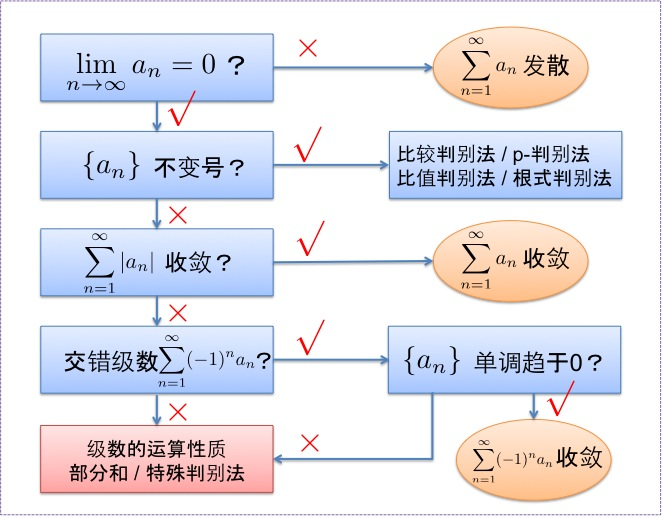
\includegraphics{./images/ch2/seriesCre/010.jpg}}
\end{center}

{\bf 例:}判断正误:
\begin{enumerate}[(1)]
  \setlength{\itemindent}{1cm}
  \item 若$a_n>0(n=1,2,\ldots)$,则\\
  \centerline{$a_1-a_1+a_2-a_2+a_3-a_3+\ldots $}
  收敛 \hfill ({$\times$})
  \item 若以上$\limn a_n=0$,则以上级数收敛 \hfill
  ({$\surd$})
  \item $\sumn a_n$收敛,$\limn b_n=1\Rightarrow\sumn a_nb_n$收敛
  \hfill ({$\times$})
  \item $\sumn a_n$部分和有界,$\limn b_n=0\Rightarrow\sumn a_nb_n$收敛
  \hfill ({$\times$})
  \item 若$\limn\df{a_n}{b_n}=1$,则若$\sumn a_n$绝对收敛,$\sumn b_n$必收敛 \hfill
  ({$\surd$})
  \item $\sumn a_n,\sumn b_n$绝对收敛$\Rightarrow\sumn (a_n+b_n)$绝对收敛 \hfill
  ({$\surd$})
  \item $\sumn a_n,\sumn b_n$条件收敛$\Rightarrow\sumn (a_n+b_n)$条件收敛 \hfill
  ({$\times$})
  \item 若$\sumn a_n^2$收敛,则$\sumn a_n^3$收敛 \hfill
  ({$\surd$})
\end{enumerate}

{\bf 例:}判断下列级数的敛散性
\begin{enumerate}[(1)]
  \setlength{\itemindent}{1cm}
  \item $\sumn\df{2^nn!}{n^n}$
  \item $\df 1{a+b}+\df 1{2a+b}+\df 1{3a+b}+\ldots\quad (a>0,b>0)$
  \item $\sumn\df{1!+2!+\ldots+n!}{n!}$
  \item $\sumn\left[\df 1n-\ln\left(1+\df 1n\right)\right]$
  \item $\sumn\df{\sqrt{n!}}{(2+\sqrt 1)(2+\sqrt 2)\ldots(2+\sqrt n)}$
  \item $\sumn\df{\sqrt{n+1}-\sqrt{n}}{n^p}\quad(p>0)$
  \item $\sumn\df{n^{n+\frac 1{\,n\,}}}{\left(n+\df 1n\right)^n}$
  \item $\sumn n!\left(\df{x}{n}\right)^n\quad (x>0)$
  \item $\sumn\df {a_n}{(1+a_1)(1+a_2)\ldots(1+a_n)}\quad(a_n\geq
	  0,n\in\mathbb{N})$
  \item $\sumn\df{n^{n+\frac 1{\,n\,}}}{\left(n+\df 1n\right)^n}$
\end{enumerate}

\newpage

\section*{课后作业}

\begin{itemize}
  \item 习题2.1:2,6(1,3),7,9
  \item 已知数列$\{a_n\}$单调递增,它的一个子列$\{a_{n_k}\}$收敛于$a$,
  证明:$\limn a_n=a$。
  \item 证明:$\sqrt[n]n\to 1\,(n\to\infty)$。
  \item 习题2.2:1(4,6),2(2,3),3,7,9,11
  \item 习题2.3:4,5,6
  \item 写出根植判别法的不等式形式,并证明。
  \item 习题2.4:1(2-4),3(3-8),5(2,4),6(1-3),8,9
  \item 习题2.5:2(1,3,6,7,8),3,7,8
\end{itemize}

{\bf 【课堂练习与思考题】}

\begin{itemize}
  \item 习题2.2:6,8,10,12,18
  \item 设$0<a_1<2$,且$(2-a_n)a_{n+1}=1\,(n\in\mathbb{N})$,
  	证明$\{a_n\}$收敛,求其极限。
  \item 设$x_1=\df 12$,$x_{n+1}=x_n^2+x_n\,(n\in\mathbb{N})$,求
	$$\limn\left(\df 1{x_1+1}+\df 1{x_2+1}+\ldots+\df
	1{x_n+1}\right)$$
  \item 已知$0<x<1$,数列$\{a_n\}$定义如下:
	$$a_1=\df x2,\;a_n=\df x2-\df{a_{n-1}^2}2.$$
	证明$\{a_n\}$收敛,并求其极限。
  \item 习题2.3:7,8 
  \item 习题2.4:10-15,17
  \item 习题2.5:4,6,10,13
\end{itemize}

\setcounter{chapter}{2}

\chapter{函数极限与连续}

\section{函数极限的概念与性质}

\subsection{函数极限的概念}

{\bf 函数极限的六种不同趋势}

\begin{itemize}
  \setlength{\itemindent}{1cm}
  \item 趋于无穷
  $$x\to\infty,\quad x\to+\infty,\quad x\to-\infty$$
  \item 趋于有限值
  $$x\to x_0,\quad x\to x_0^+,\quad x\to x_0^-$$
\end{itemize}

{\bf 思考:} $\limn f(n)=A\Leftrightarrow\limx{+\infty}f(x)=A$?($\times$)

\subsubsection{趋于无穷时的函数极限}

{\bf 定义3.1.1}
\begin{enumerate}[(1)]
  \setlength{\itemindent}{1cm}
  \item $\limx{+\infty}f(x)=A\Leftrightarrow\forall \e>0,\exists X,\forall
  x>X,|f(x)-A|<\e$
  \item $\limx{-\infty}f(x)=A\Leftrightarrow\forall \e>0,\exists X,\forall
  x<X,|f(x)-A|<\e$
  \item $\limx{\infty}f(x)=A\Leftrightarrow\forall \e>0,\exists X,\forall
  |x|>X,|f(x)-A|<\e$
\end{enumerate}

{\bf 注:}趋于无穷的函数极限存在,意味着函数存在{\bf 水平渐近线},例如
$$y=\arctan x$$

\begin{center}
	\resizebox{!}{6cm}{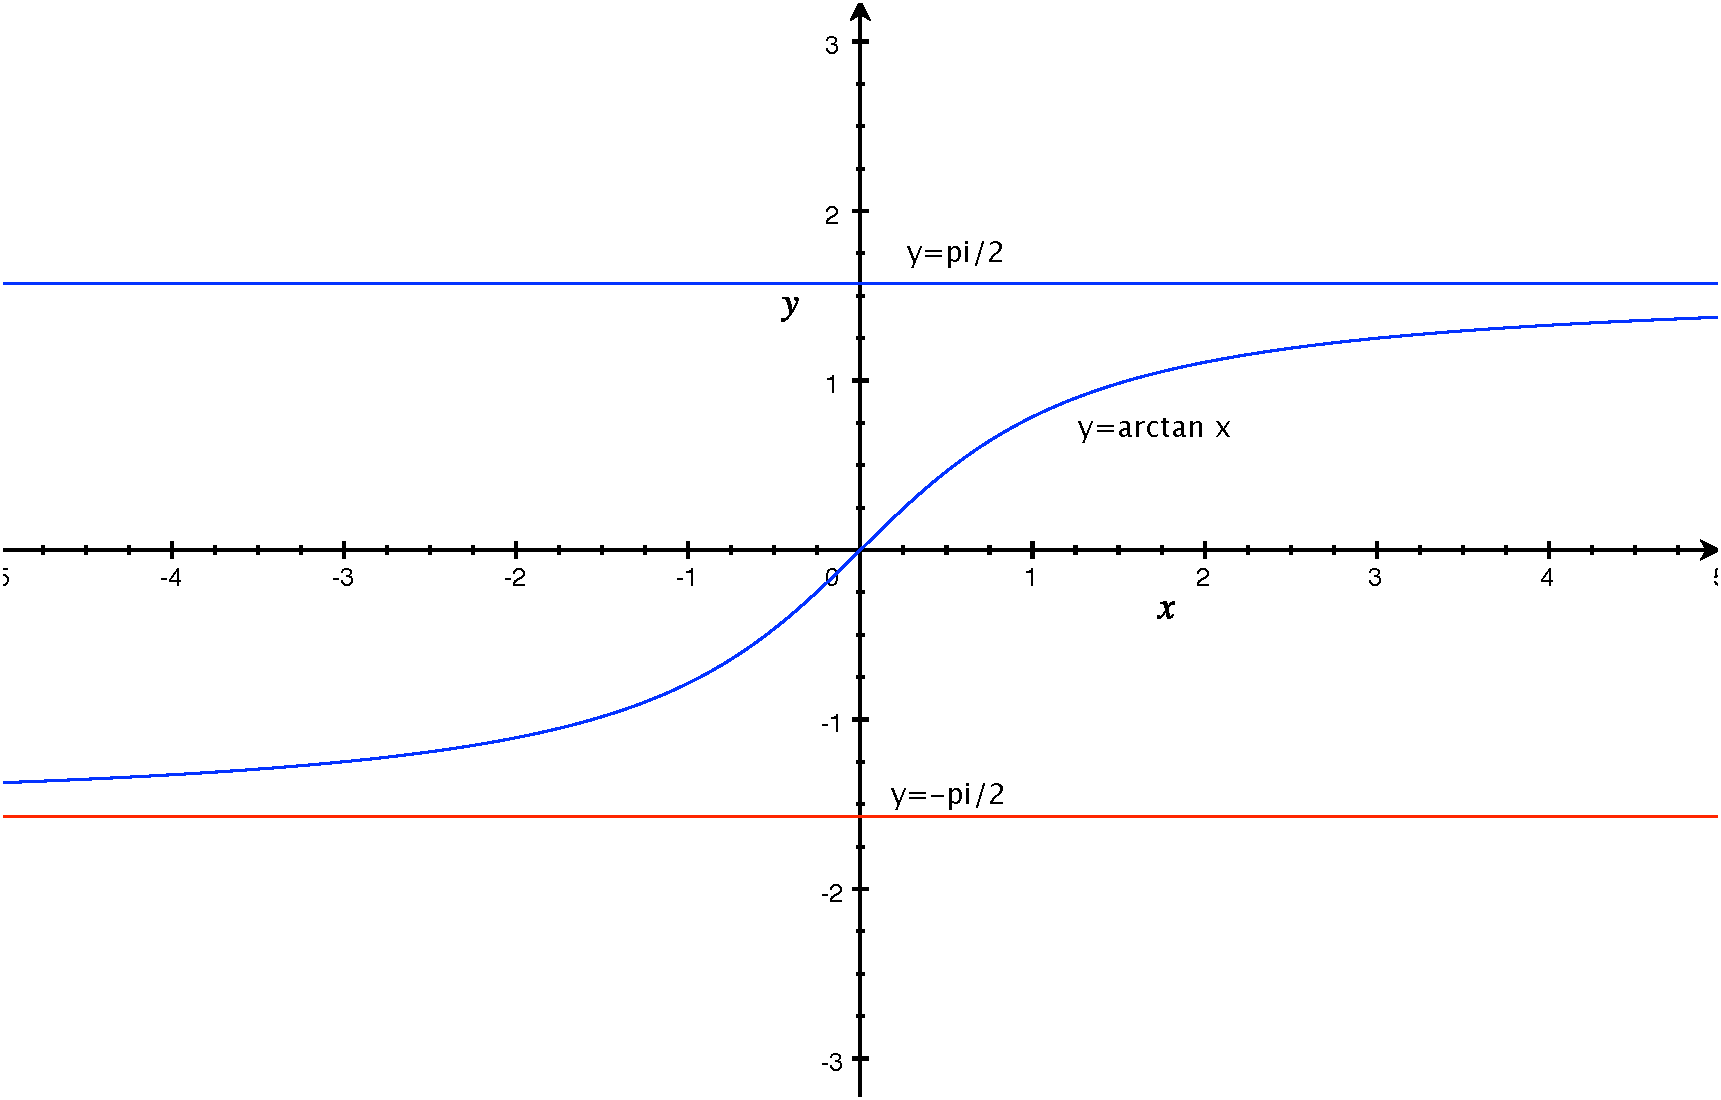
\includegraphics{./images/ch3/arctan.pdf}}
\end{center}

{\bf 例:}证明$\limx{+\infty}\df1{\sqrt x}=0$.

{\bf 注:}和$\limn a_n=a$的定义做类比,理解(1),然后推广到(2),(3)。特别是有关的性质,如
\begin{itemize}
  \setlength{\itemindent}{1cm}
  \item $A$必须是确定值
  \item $\e$可以任意小
  \item $X$要充分大(或小)
  \item 不等式右端可以乘以某个常数$C$
\end{itemize}

{\bf 定义3.1.2}
\begin{enumerate}[(1)]
  \setlength{\itemindent}{1cm}
  \item $\limx{x_0}f(x)=A\Leftrightarrow\forall \e>0,\exists\delta>0,\forall
  x\in U_0(x_0,\delta),|f(x)-A|<\e$
  \item $\limx{x_0^+}f(x)=A\Leftrightarrow\forall \e>0,\exists\delta>0,\forall
  x\in(x_0,x_0+\delta),|f(x)-A|<\e$
  \item $\limx{x_0^-}f(x)=A\Leftrightarrow\forall \e>0,\exists\delta>0,\forall
  x\in(x_0-\delta,x_0),|f(x)-A|<\e$
\end{enumerate}

{\bf 例}(习题3.1-1)根据图形判断极限的存在性
\begin{center}
	\resizebox{!}{4cm}{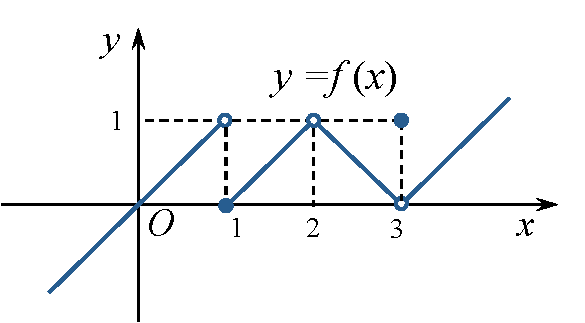
\includegraphics{./images/ch3/limxf.pdf}}
\end{center}
\begin{enumerate}[(1)]
  \setlength{\itemindent}{1cm}
  \item $\limx{1}f(x)$\underline{不存在}
  \item $\limx{2}f(x)$\underline{$=1$}
  \item $\limx{1}f(x)$\underline{$=0$}
\end{enumerate}

{\bf 思考:}
\begin{itemize}
  \setlength{\itemindent}{1cm}
  \item 为什么在定义中要求$0<|x-x_0|<\delta$,而不是$|x-x_0|<\delta$?
  {\it (因为极限表示一种趋势,与函数在该点处的取值无关)}
  \item $f(x_0+0),f(x_0-0)$与$f(x_0)$是何关系?
  {\it(前两者分别表示左右极限,最后一个是函数值,三者相互无关)}
\end{itemize}

{\bf 例:}证明
\begin{enumerate}[(1)]
  \setlength{\itemindent}{1cm}
  \item $\limx{1}\df1x=1$
  \item $\limx{x_0}\sin x=\sin x_0$
\end{enumerate}

\begin{shaded}
	{\bf 【函数极限的反面说法】}
	
	\begin{itemize}
	  \item 当$x\to x_0$时$f(x)$不以$A$为极限 
	    $$\exists\e_0>0,\forall\delta>0, \exists x^*\in
	    U_0(x_0,\delta),|f(x^*)-A|\geq\e_0$$ 
	  \item 当$x\to x_0$时$f(x)$无极限
		$$\forall A\in\mathbb{R},\exists\e_0>0,\forall\delta>0, \exists x^*\in
	    U_0(x_0,\delta),|f(x^*)-A|\geq\e_0$$ 
	\end{itemize}
	
	{\bf 例:}证明:Dirichlet函数在任意点处无极限。
\end{shaded}

\subsection{函数极限的基本性质}

\subsubsection{【唯一性】}

{\bf 定理3.1.2:}函数极限若存在,必唯一。

\subsubsection{【有界性】}

{\bf 定理3.1.3:}
\begin{enumerate}[(1)]
  \setlength{\itemindent}{1cm}
  \item 若$\limx{+\infty}f(x)=A$,则$f(x)$当$x$充分大时有界
  \item 若$\limx{x_0}f(x)=A$,则$f(x)$在$x_0$的某去心领域内有界
\end{enumerate}

{\bf 注意:}函数极限有界性和数列极限有界性的叙述存在很大差异!!\ps{数列极限中的数列整体有界,
是由数列自身的“稀疏”特性所决定的}

\subsubsection{【保号性】}

{\bf 定理3.1.4:}
\begin{enumerate}[(1)]
  \setlength{\itemindent}{1cm}
  \item 若$\limx{+\infty}f(x)=A>0$,则当$x$充分大时,$f(x)>0$
  \item 若$\limx{x_0}f(x)=A>0$,则在$x_0$的某去心领域内,$f(x)>0$
\end{enumerate}

\subsubsection{【四则运算】}

{\bf 定理3.2.1:}若函数极限存在,则极限运算可以和四则运算交换次序。

{\bf 注:}把握两点
\begin{itemize}
  \setlength{\itemindent}{1cm}
  \item 有限次四则运算
  \item 可以推广到初等函数
\end{itemize}

{\bf 课堂思考:}
\begin{enumerate}[(1)]
  \setlength{\itemindent}{1cm}
  \item 若$x\to x_0$时,$f(x)$有极限,$g(x)$无极限,则当$x\to x_0$时,以下哪些函数必无极限:
  $$f(x)g(x),\quad [g(x)]^2,\df{g(x)}{f(x)}, f(x)+g(x)$$ 
  \item 若$\limx{x_0}g(x)=A,\lim\limits_{u\to A}f(u)=B$,是否必有
  $$\limx{x_0}f[g(x)]=B\;?$$
  \item 若$\limx{x_0}f(x)g(x)=0$,则当$x\to
  x_0$时, $f(x),$ $g(x)$之一必趋于$0$ ({$\times$})
\end{enumerate}

{\bf 例:}设$\limx{x_0}f(x)=A$,用定义证明:$\limx{x_0}[f(x)]^3=A^3$

\section{函数极限的判敛}

\subsection{复合函数的极限}

{\bf 定理3.2.2:}设有复合函数$y=f[g(x)]$,其中
$$\limx{x_0}g(x)=u_0,\quad\lim\limits_{u\to u_0}f(u)=A,$$
在$x_0$附近$g(x)\ne u_0$,则
$$\limx{x_0}f[g(x)]=A.$$

{\bf 注:}
\begin{itemize}
  \setlength{\itemindent}{1cm}
  \item 直观理解:若相关极限都存在,则极限运算可以和函数运算交换次序
  \item 为什么要求“在$x_0$附近$g(x)\ne u_0$”?{\it (因为$f(x)$可能在$x_0$处无定义)}
  \item 可以类似地推广到$x\to\infty$的情形
\end{itemize}

\subsection{函数极限与数列极限的关系}

{\bf 定理3.2.3}(Hiene定理)$\limx{\Delta}f(x)=A\Leftrightarrow
$若数列$\{x_n\}$满足:$x_n\to \Delta(n\to$ $\infty)$,则
$$\limn f(x_n)=A$$

\begin{itemize}
  \setlength{\itemindent}{1cm}
  \item 以上$\Delta$对应于函数极限的六种不同趋势 
  \item {\bf 用途一:}证明极限不存在性
  \item {\bf 用途二:}利用函数极限计算对应的数列极限
\end{itemize}

{\bf P118-例8:}证明:$f(x)=\sin\df 1x$当$x\to 0$时无极限。

{\bf 例}(习题3.2-7)证明Dirichlet函数在任意点处无极限。

{\bf 例:}设在$(0,+\infty)$上,恒有$f(x^2)=f(x)$,且
$$\limx{0^+}f(x)=\limx{+\infty}f(x)=f(1)$$
证明:$f(x)=f(1)\,(x\in(0,+\infty))$

\subsection{夹逼定理}

{\bf 定理3.2.5:}设在$x_0$的某邻域内,恒有
$$\varphi(x)\leq f(x)\leq\psi(x), $$
且$\limx{x_0}\varphi(x)=\limx{x_0}\psi(x)=A$,则
$$\limx{x_0}f(x)=A.$$

{\bf P120-例9}(重要极限一)证明:
$$\limx{\infty}\left(1+\df 1x\right)^x=e$$

\begin{shaded}
{\bf 例}(另一种证明)令$f_u=x^ue^{-x}(x\geq 0)$,对于确定的$u$,证明:
\begin{enumerate}[(1)]
  \setlength{\itemindent}{1cm}
  \item $f_u(x)$在$x=u$处取最大值;
  \item 由$f_u(x)>f_u(u+1)$和$f_{u+1}(u+1)>f_u(u)$推出
  $$\left(\df{u+1}u\right)^u<e<\left(\df{u+1}u\right)^{u+1}$$
  \item $\df u{u+1}e<\left(\df{u+1}u\right)^u<e$,由此推出
  $$\limx{+\infty}\left(1+\df 1u\right)^u=e$$
\end{enumerate}
\end{shaded}

{\bf 例:}{\it 这些都是重要极限的应用,须牢记有关结果!!!}
\begin{enumerate}[(1)]
  \setlength{\itemindent}{1cm}
  \item $\limx{0}(1+x)^{1/x}$ 
  \item $\limx 0(1+\sin x)^{1/\sin x}$ 
  \item $\limx 0\df{\ln(1+ax)}{x}$
  \item $\limx 0\df{e^{ax}-1}{x}$ 
  \item $\limx 0\df{a^x-1}{x}(a>0)$ 
  \item $\limn n(\sqrt[n]{a}-1) (a>0)$ 
\end{enumerate}

{\bf P121-例11}(重要极限二)证明:
$$\limx{0}\df {\sin x}x=1$$

{\bf [hint]:}
\begin{center}
	\resizebox{!}{5cm}{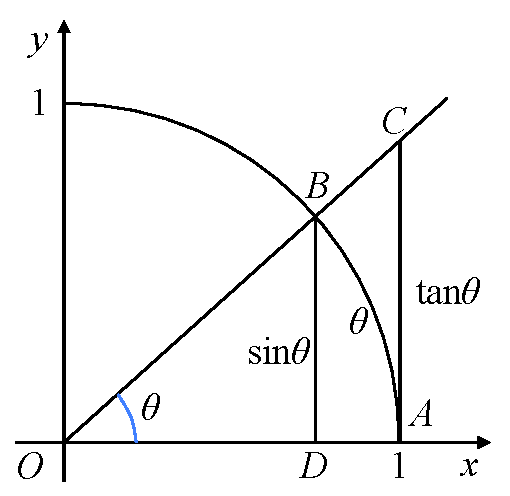
\includegraphics{./images/ch3/xsintan.pdf}}
\end{center}

如图,显然弧$AB$的长度大于直线$BD$,即$\sin\theta<\theta$;又扇形$ABO$的面积$\df12\theta$
小于三角形$ACO$的面积$\df12\tan\theta$,从而$\theta<\tan\theta$

{\bf 例:}{\it 牢记!!!}
\begin{enumerate}[(1)]
  \setlength{\itemindent}{1cm}
  \item $\limx{0}\df{\sin\sin x}{\sin x}$ 
  \item $\limx 0\df{1-\cos x}{x^2}$ 
  \item $\limx 0\df{\sin mx}{\sin nx}(n\ne 0)$
  \item $\limx 0\df{\tan x}{x}$
  \item $\limx a\df{\sin x-\sin a}{x-a}$
\end{enumerate}

{\bf 例:}设$f(x)=\sum\limits_{i=1}^na_i\sin
ix$,其中$a_i(i=1,2,\ldots,n)$为常数,且对任意$x\in\mathbb{R}$, $|f(x)|\leq |\sin x|$,证明:
$$\left|a_1+2a_2+\ldots+na_n\right|\leq 1$$

\section{无穷大、无穷小和函数的渐近线}

\subsection{无穷大和无穷小}

{\bf 定义3.3.1:}$f(x)$是$x\to\Delta$时的无穷小$\Leftrightarrow\limx{\Delta}f(x)=0$

{\bf 注:}$\Delta$可任意代表$\infty,\;+\infty,\;-\infty,\;x_0,\;x_0^+,\;x_0^-$之一

{\bf 定理3.3.1-3.3.2}(无穷小的性质)
\begin{enumerate}[(1)]
  \setlength{\itemindent}{1cm}
  \item $\limx{\Delta}f(x)=A\in\mathbb{R}\Leftrightarrow
  f(x)-A$是$x\to\Delta$时的无穷小
  \item 同一过程的有界函数中与无穷小之积仍为该过程中的无穷小
  \item 在同一过程中的有限个无穷小之和(积)仍为该过程中的无穷小
\end{enumerate}

{\bf 定义3.3.2:}$f(x)$是$x\to\Delta$时的无穷大$\Leftrightarrow\limx{\Delta}\df 1{f(x)}=0$,
可记为:
$$\limx{\Delta}f(x)=\pm\infty$$

{\bf 注:}无穷大有正负之分!!

{\bf 【渐近线】:}$x\to x_0$时的无穷大意味着存在铅直渐近线;$x\to\pm\infty$时的无穷大
{\it 可能}意味着存在斜渐近线

{\bf P129-例4:}证明:$x+\sin x$是$x\to\infty$时的无穷大

{\bf 定理3.3.3:}在$x\to\Delta$的同一过程中:
\begin{enumerate}[(1)]
  \setlength{\itemindent}{1cm}
  \item 有界函数与无穷大之和仍为无穷大
  \item 有限个无穷大之乘积仍为无穷大({\it 但可能反号})
\end{enumerate}

{\bf 例:}证明:$f(x)=a_0x^n+a_1x^{n-1}+\ldots+a_n(n\in\mathbb{N})$
是$x\to\infty$时的无穷大,其中:$a_0,a_1,\ldots,a_n\in\mathbb{R},a_0\ne 0$

\subsection{无穷小的比较}

{\bf 定义3.3.3:}设$y_1,y_2$均为$x\to\Delta$时的无穷小,
$\limx{\Delta}\df{y_1}{y_2}=A$为常数
\begin{enumerate}[(1)]
  \setlength{\itemindent}{1cm}
  \item $A=0$,称$y_1$为$y_2$当$x\to\Delta$时的{\bf 高阶(高级)无穷小},记为:
  $$y_1=\circ( y_2)\;(x\to\Delta)$$
  \begin{itemize}
    \item {\bf 无穷小}记为:
    $$y_1=\circ(1)\;(x\to\Delta)$$
  \end{itemize}
  \item $A\ne 0$,称$y_1$为$y_2$当$x\to\Delta$时的{\bf 同阶(同级)无穷小},记为:
  $$y_1=\mathrm{O}( y_2)\;(x\to\Delta)$$
  \item $A=1$,称$y_1$为$y_2$当$x\to\Delta$时的{\bf 等价无穷小},记为:
  $$y_1\sim y_2\;(x\to\Delta)$$
\end{enumerate}

{\bf 注意:}所有的无穷小都必须是和$x$的某个变化趋势相关的!!!

\begin{shaded}
	{\bf 【高阶无穷小的计算】}
	当$x\to 0$时
	\begin{enumerate}[(1)]
  	  \setlength{\itemindent}{1cm}
	  \item $x^n=\circ(x^m)\;(m<n)$ 
	  \item $\circ(x^n)=x^n\circ(1)$ 
	  \item $x^n\circ(x^m)=\circ(x^{m+n})$ 
	  \item $\circ(x^n)+\circ(x^m)=\circ(x^n)\;(m\geq n)$ 
	  \item $C\circ(x^n)=\circ(x^n)\;(C\in\mathbb{R}\mbox{为常数})$ 
	  \item $\circ(x^n)\circ(x^m)=\circ(x^{m+n})$
	\end{enumerate}
\end{shaded}

\subsection{(等价)无穷小代换}

{\bf 等价无穷小的基本性质:}
\begin{itemize}
  \setlength{\itemindent}{1cm}
  \item {\bf 自反性:} $y\sim y$ 
  \item {\bf 对称性:} $y_1\sim y_2\Rightarrow y_2\sim y_1$ 
  \item {\bf 传递性:} $y_1\sim y_2,y_2\sim y_3\Rightarrow y_1\sim y_3$ 
\end{itemize}

{\bf 定理3.3.4:}设$y_1\sim y_2\;(x\to\Delta)$,则
$$\limx{\Delta}y_1y_3=A\Leftrightarrow\limx{\Delta}y_2y_3=A$$

{\bf 注:}极限“乘法因子”中的等价无穷小可相互替代

{\bf 【常用无穷小代换】}:$x\to 0$时
\begin{enumerate}[(1)]
  \setlength{\itemindent}{1cm}
  \item $x\sim \sin x\sim \tan x$ 
  \item $x \sim\arcsin x\sim\arctan x$ 
  \item $1-\cos x\sim \df 12 x^2$ 
  \item $(1+x)^a-1\sim ax$ 
  \item $\ln(1+x)\sim x$ 
  \item $a^x-1\sim x\ln a\;(a>0)$
\end{enumerate}

{\bf 例:}计算极限
\begin{enumerate}[(1)]
  \setlength{\itemindent}{1cm}
  \item $\limx{0}\df{\arctan x}{\sin 4x}$ 
  \item $\limx{0}\df{\ln\cos ax}{\ln\cos bx}$ 
  \item $\limx{0}\df{\cos x(e^{\sin x}-1)^4}{\sin^2 x(1-\cos x)}$ 
  \item $\limx{0}\df{\sin x-\tan x+x^3}{\sin^3 x}$
\end{enumerate}

{\bf 极限中的“加法因子”不能进行无穷小代换!}

\subsection{斜渐近线}

若$y=f(x)$当$x\to+\infty$时以$y=kx+b$为斜渐进线,则有
$$k=\limx{+\infty}\df{f(x)}{x}=k,\quad b=\limx{+\infty}[f(x)-kx]$$

{\bf 例:}求曲线$y^2-x^2=2x$的渐近线。

{\bf P135-例10:}求函数$f(x)=\df{2x^2-3}{x+1}$的渐近线。

\section{函数的连续性}

\subsection{定义}

{\bf 定义3.4.1:}函数$f(x)$在$x_0$连续:
$$\limx{x_0}f(x)=f(x_0)$$

\begin{itemize}
  \item $f(x)$在$x_0$有定义 
  \item $\limx{x_0}f(x)$存在 
  \item $f(x_0)=f(x_0+0)=f(x_0-0)$
\end{itemize}

{\bf 注:}必要时,可以只考虑函数在某点一侧的连续性,即所谓左(右)连续,
参见教材定义3.4.2-3

{\bf 例:}证明:$f(x)=xD(x)$只在$x=0$处连续。

{\bf P140-例3:}设$f(x)$在$(-\infty,+\infty)$上有定义,
且对任意$x,y\in (-\infty,+\infty)$,有
$$f(x+y)=f(x)+f(y),$$
则$f(x)$在$(-\infty,+\infty)$上连续,当且仅当$f(x)$在$x=0$连续。

{\bf 定义3.4.4:}设$x_0$是$f(x)$的间断点(不连续点),对其分类定义如下:
\begin{enumerate}[(1)]
  \setlength{\itemindent}{1cm}
  \item {\bf 第一类间断点:}$f(x_0+0),f(x_0-0)$均存在
  \begin{itemize}
    \item {\bf 跳跃间断点:}$f(x_0+0)\ne f(x_0-0)$
    \item {\bf 可去间断点:}$f(x_0)$无定义,或
    $$f(x_0)\ne f(x_0+0)=f(x_0-0)$$
  \end{itemize}
  \item {\bf 第二类间断点:}$f(x_0+0),f(x_0-0)$不同时存在
  \begin{itemize}
    \item {\bf 无穷间断点:}某个单侧极限趋于无穷
    \item {\bf 振荡间断点:}某个单侧极限不存在
  \end{itemize}
\end{enumerate}

\subsection{基本性质}

{\bf 定理3.4.1-3.4.4:}
\begin{enumerate}[(1)]
  \setlength{\itemindent}{1cm}
  \item {\bf 四则运算:} 四则运算仍保持函数的连续性 
  \item {\bf 复合函数:} 连续函数的函数运算可以和极限运算交换次序 
  \item {\bf 反函数:} 连续函数的反函数也连续 
  \item {\bf 初等函数:} 初等函数在其定义域内连续
\end{enumerate}

\subsection{连续函数在有界闭区间上的性质}

\subsubsection{【最值定理】}

{\bf 定理3.4.5:}设$f(x)\in C[a,b]$,则$f(x)$在$[a,b]$上可取到最大和最小值。

{\bf 推论:}设$f(x)\in C[a,b]$,则$f(x)$在$[a,b]$上有界。

{\bf 例:}设$f(x)\in C[a,+\infty)$,且$\limx{+\infty}f(x)$存在,
则$f(x)$在$[a,+\infty)$上有界。

\subsubsection{【介值定理】}

{\bf 定理3.4.6:}设$f(x)\in C[a,b]$,$M,m$分别为$f(x)$在$[a,b]$上的最大和最小值,
则对任意$\gamma\in[m,M]$,存在$\xi\in[a,b]$,使得$f(\xi)=\gamma$。

{\bf 推论}(零值定理/零点存在性)
设$f(x)\in C[a,b]$,且$f(a)f(b)<0$,则$f(x)$在$[a,b]$上必有零点。

{\bf 推论'}(零点存在性定理的推广)
\begin{enumerate}[(1)]
  \setlength{\itemindent}{1cm}
  \item 设$f(x)\in C(a,b)$,且$f(a+0)f(b-0)<0$,则$f(x)$在$(a,b)$内有零点。 
  \item 设$f(x)\in C(-\infty,+\infty)$,且$f(-\infty)f(+\infty)<0$,
  则$f(x)$在$(-\infty,+\infty)$内有零点。
\end{enumerate}

{\bf 例:}设$a_0\ne 0$,证明:以下方程至少有一个实根
$$a_0x^{2n+1}+a_1x^{2n}+\ldots+a_{2n}x+a_{2n+1}=0.$$

{\bf 例:}设$G$是第一象限内的一个有界区域(其边界为连续的简单闭曲线),$ABCD$表示
它的一个外接矩形。矩形的一条边与$x$轴的夹角记为$\theta$,如果对于任意$\theta\in
[0,\pi/2]$,$G$总可以被某个外接矩形所围,证明:至少存在某个$\theta_0\in[0,\pi/2]$,
使得与之对应的外接矩形恰好为正方形。({\it 推论:任一平面有界区域都可以内接于某个正方形})

\begin{center}
	\resizebox{!}{6cm}{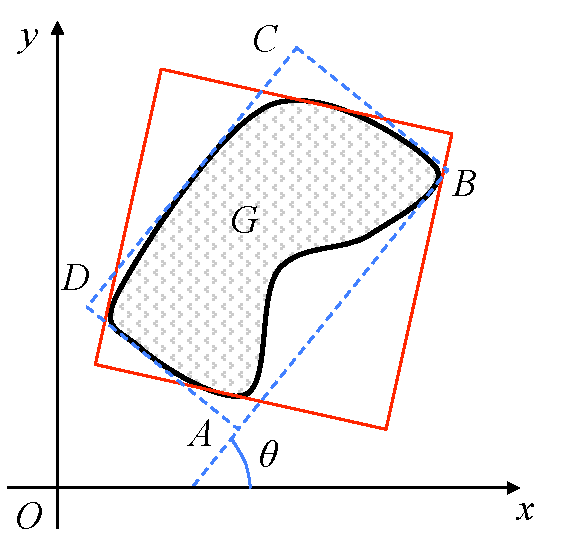
\includegraphics{./images/ch3/sqOut.pdf}}
\end{center}

{\bf [hint]:}记$l_1(\theta),l_2(\theta)$分别为$AB$和$BC$的长度,显然
$$l_1(0)=l_2(\pi/2),\quad l_2(0)=l_1(\pi/2).$$
令$f(\theta)=l_1(\theta)-l_2(\theta)$,由介值定理可以证明$f(\theta)$存在零点。

{\bf 例:}证明:给定任意平面有界区域,以及一个向量,一定存在一条与该向量平行的直线
平分该区域。

{\bf 例:}证明:给定任意平面有界区域,一定存在两条相互垂直的直线,将其四等分。

{\bf [hint]:} 设其中一条直线的极角为$\theta$,则另一条的为$\theta+\pi/2$。
分别记两条直线为$l_{\theta}$和$l_{\theta+\pi/2}$,显然可以使得二者都平分给定区域。
设此时四个区域的面积按顺时针方向依次为$S_1,S_2,S_3,S_4$,且由平分可满足
$$A_1+A_2=A_3+A_4,\quad A_1+A_4=A2+A_3,$$

\begin{center}
	\resizebox{!}{6cm}{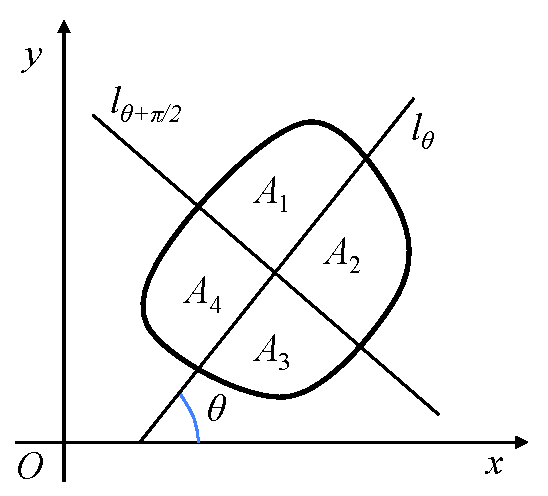
\includegraphics{./images/ch3/4cut.pdf}}
\end{center}

由此可得
$$A_1=A_3,\quad A_2=A_4.$$
进而,只需适当取$\theta$,使得$A_1=A_2$即可。

记$f(\theta)=A_1(\theta)-A_2(\theta)$,不妨设$f(0)>0$,从而
$$f(\pi/2)=A_1(\pi/2)-A_2(\pi/2)=A_4(0)-A_1(0)=A_2(0)-A_1(0)=-f(0)<0,$$
由介值定理,即证。

{\bf 例:}任意金属圆环上,总存在相对的两点温度相同。
({\it 圆环可以看成赤道,温度即为两点的气温})

\newpage

\section*{课后作业}

\begin{itemize}
  \item 习题3.1:4(1,3),6,7,10
  \item 习题3.2:2,3,5,6
  \item 习题3.3:2,4,5,8,9,10
  \item 习题3.4:4,5(1-3),9,14,15,17
\end{itemize}

{\bf 【课堂练习与思考题】}
\begin{itemize}
  \item 习题3.1:11,12
  \item 习题3.2:4,7
  \item 证明:$$\limn\left\{\lim\limits_{m\to\infty}\left[\cos^{2m}(n!\pi
	x)\right]\right\}=D(x)$$
	其中$D(x)$为Dirichlet函数
  \item 自学3.3.3节:渐近线 
  \item 习题3.3:1,6,12,13
  \item  计算极限
	\begin{enumerate}[(1)]
% 	  \setlength{\itemindent}{1cm}
	  \item $\limx{+\infty}(\sqrt{x^2+x+1}-\sqrt{x^2+x-1})$ 
	  \item $\limx{0}\df{\sqrt[3]{1+x}-1}{x}$ 
	  \item $\limx{0}\df{\sqrt{1-\cos x^2}}{1-\cos x}$ 
	  \item $\limx{0}\df{1-\cos x\cos 2x}{1-\cos x}$
	  \item $\limx{\pi /4}(\tan x)^{\tan 2x}$ 
	  \item $\limx{0}\left(2e^{\frac{x}{x+1}}-1\right)^{\frac{x^2+1}{x}}$ 
	  \item $\limx{+\infty}\left(\sqrt{x^2+x}-\sqrt[3]{x^3+x^2}\right)=
	  \limx{+\infty}x\left(1+\df1x\right)^{\df13}\left[\left(
	  1+\df1x\right)^{\df16}-1\right]=\df16$ 
	  \item $\limx{+\infty}\left(\df{x^2-1}{x^2+1}\right)^{x^2}$
	  \item $\limx{0}\left(\df{a^x+b^x+c^x}{3}\right)^{1/x}\,(a,b,c>0)$ 
	  \item $\limx{0}\left(\df{a^{x+1}+b^{x+1}+c^{x+1}}{a+b+c}\right)^{1/x}
	  \,(a,b,c>0)$ 
	  \item $\limx{0}\df{\tan(\tan x)-\sin(\sin x)}{\tan x-\sin x}$
	\end{enumerate}
  \item 习题3.4:1,3,13,16,19
  \item 设$a_1<a_2<\ldots<a_n$,证明以下方程有$n-1$个实根
	$$\df 1{x-a_1}+\df 1{x-a_2}+\ldots+\df 1{x-a_n}=0.$$
\end{itemize}

% \setcounter{chapter}{3}

\chapter{导数与不定积分}

\section{导数的概念}

\subsection{函数在一点处的导数}

{\bf 定义4.1.1:}函数$y=f(x)$在$x_0$的某领域内有定义,若
$$\limdx\df{f(x_0+\dx)-f(x_0)}{\dx}$$
存在, 则称其为{\it $f(x)$在$x_0$处的导数}, 记为
$$f\,'(x_0),\quad \left.\df{\d y}{\d x}\right|_{x=x_0},
\quad y'_x|_{x=x_0}$$

{\bf 例1:}假设$f\,'(x_0)$存在,则
\begin{enumerate}[(1)]
  \setlength{\itemindent}{1cm}
  \item $\limdx\df{f(x_0-\Delta x)-f(x_0)}{\Delta
  x}=$ \underline{\quad{$-f\,'(x_0)$}\quad} 
  \item $\lim\limits_{h\to 0}\df{f(x_0+2h)-f(x_0)}{h}=$
   \underline{\quad{$2f\,'(x_0)$}\quad} 
  \item $\lim\limits_{h\to 0}\df{f(x_0+h)-f(x_0-h)}{h}=$ 
  \underline{\quad{$2f\,'(x_0)$}\quad}
\end{enumerate}

{\bf 思考:}若以上某个极限存在,是否就意味着$f(x)$在$x_0$可导?

\subsubsection{【导数的物理/几何意义】}

\begin{itemize}
  \setlength{\itemindent}{1cm}
  \item {\it 切线斜率:}
  $$k(x_0)=\lim\limits_{x\to x_0}\df{f(x)-f(x_0)}{x-x_0}$$
  \item {\it 瞬时速度:}
  $$v(t_0)=\lim\limits_{t\to t_0}\df{S(t)-S(t_0)}{t-t_0}$$
\end{itemize}

{\bf 导数:函数关于自变量的相对变化率!}\ps{当自变量发生变化时,函数值发生的相应变化与之的比率}

{\bf 例:}已知函数$f(x)$在点$x_0$处可导,求曲线$y=f(x)$在该点的切线和法线方程。

{\bf 思考:}可导等价于有切线吗?(否)

{\bf P156-例1:}讨论函数$f(x)=\sqrt[3]x$在点$x=0$是否可导?

\subsubsection{【导数存在的条件】}

{\bf 定理4.1.1:}$f(x)$在$x_0$可导,当且仅当在该点的左、右导数存在且相等。

{\bf 定理:}初等函数在其定义域内是处处可导的。

{\bf 定理4.1.2:}$f(x)$在一点可导,则一定在该点连续。

{\bf P164-例8:}确定常数$a,b$的值,使得函数
$$f(x)=\left\{\begin{array}{ll}ax+b,& x>0\\
e^x,& x\leq 0\end{array}\right.$$
在$x=0$可导。

{\bf 例:}设$f(x)=\left\{\begin{array}{ll}
\df{1-\sqrt{1-x}}{x}, & x<0,\\
a+bx, & x\geq 0
\end{array}\right.$,求$a,b$使$f(x)$处处可导。

{\bf 例:}问题讨论
\begin{enumerate} 
  \setlength{\itemindent}{1cm}
  \item 若$f(x),g(x)$在$x_0$均不可导,是否$f(x)+g(x),$ $f(x)g(x)$必不可导?
  ({$\times$}) 
  \item 若对任意$x\in (a,b)$,恒有$f(x)<g(x)$,且$f(x),g(x)$均在$(a,b)$内
  可导,问是否必有$f\,'(x)<g'(x)$? ({$\times$}) 
  \item 若$f(x)$在$\mathbb{R}$上可导,且$\limx{+\infty}f(x)=\infty$,是否
  必有$\limx{+\infty}f\,'(x)=\infty$? ({$\times$})
  \item 若$f(x)$在$(a,b)$内可导,且$\limx{a^+}f(x)=\infty$,是否
  必有$\limx{a^+}f\,'(x)=\infty$? ({$\times$}) 
  \item 若$f(x)$可导且为奇(偶)函数,则$f\,'(x)$也有奇偶性? ({$\surd$}) 
  \item 若$f(x)$可导且为周期函数,则$f\,'(x)$也是周期函数? ({$\surd$})
\end{enumerate}

\subsection{导函数}

{\bf 例}({\it 一些常用函数的导函数})
\begin{enumerate}[(1)]
  \setlength{\itemindent}{1cm}
  \item $f(x)=C\;(C\mbox{为常数})$ \hfill $f\,'(x)=0$ 
  \item $f(x)=x^n\;(n\in\mathbb{Z})$ \hfill $f\,'(x)=nx^{n-1}\,(n\ne
  0)$ 
  \item $f(x)=e^x$ \hfill $f\,'(x)=e^x$ 
  \item $f(x)=\ln x$ \hfill $f\,'(x)=\df 1x$ 
  \item $f(x)=\sin x$ \hfill $f\,'(x)=\cos x$ 
  \item $f(x)=\cos x$ \hfill $f\,'(x)=-\sin x$
\end{enumerate}

\section{导数的计算}

\subsection{四则运算的求导法则}

{\bf 定理4.2.1:}设$u(x),v(x)$均在$x$可导,则
\begin{enumerate}[(1)]
  \setlength{\itemindent}{1cm}
  \item $[u(x)\pm v(x)]'=u'(x)\pm v'(x)$ 
  \item $[u(x)v(x)]' =u'(x)v(x)+u(x)v'(x)$ 
  \item $\left[\df{u(x)}{v(x)}\right]'
  =\df{u'(x)v(x)-u(x)v'(x)}{v^2(x)}\;(v(x)\ne 0)$
\end{enumerate}

{\bf P172-例2-4:}计算以下函数的导函数
\begin{enumerate}[(1)]
  \setlength{\itemindent}{1cm}
  \item $f(x)=2x^3+3x-4x+5-\df 6x$ 
  \item $f(x)=e^x\sin x$ 
  \item $f(x)=\df{x-1}{x+1}$ 
  \item $f(x)=\df 1{\ln x}$ 
  \item $f(x)=\tan x$ \hfill $f\,'(x)=\sec^2 x$ 
  \item $f(x)=\sec x$ \hfill $f\,'(x)=\sec x\tan x$
\end{enumerate}

\subsection{反函数求导法则}

{\bf 定理4.2.2:}设$y=f(x)$是$x=\varphi(y)$的反函数,
若$x=\varphi(y)$在$y$处可导,且$\varphi'(x)\ne 0$,则
$y=f(x)$在点$x=\varphi(y)$处可导,且
$$f\,'(x)=\df{1}{\varphi'(y)}$$

{\bf P174-例7-8:}计算下列函数的导函数
\begin{enumerate}[(1)]
  \setlength{\itemindent}{1cm}
  \item $f(x)=\arcsin x$ \hfill $f\,'(x)=\df{1}{\sqrt{1-x^2}}$ 
  \item $f(x)=\arctan x$ \hfill $f\,'(x)=\df{1}{1+x^2}$
\end{enumerate}

\subsection{复合函数的求导法则}

{\bf 定理4.2.3}({\it 链式法则})设函数$u=\varphi(x)$在$x$处可导,
函数$y=f(u)$在$u=\varphi(x)$处可导,则复合函数$y=f[\varphi(x)]$
在$x$处可导,且
$$y'_x=f\,'(u)\varphi'(x)$$

{\bf P176-例5:}计算下列函数的导函数
\begin{enumerate}[(1)]
  \setlength{\itemindent}{1cm}
  \item $y=a^x\;(a>0,a\ne 1)$ \hfill $y'=a^x\ln a$ 
  \item $y=x^a$ \hfill $y'=ax^{a-1}$
\end{enumerate}

{\bf P176-例10-19:}计算下列函数的导函数
\begin{enumerate}[(1)]
  \setlength{\itemindent}{1cm}
  \item $y=e^{x^2}$ 
  \item $y=\sin (3x+2)$ 
  \item $y=\cos^2(1-2x)$ 
  \item $y=\ln\sin e^{-x}$ 
  \item $y=(1-30x)^{50}$ 
  \item $y=\ln(1+x^2)$ 
  \item $y=e^{\sqrt{1-3x}}$ 
  \item $y=x^x$ 
  \item $y=e^{\tan\frac 1x}$
\end{enumerate}

{\bf P180-例20:}设$f(x)$可导,且$f\,'\left(\df{\pi}{4}\right)=1$,求
$$\varphi(x)=f\left(\arctan\df{1+x}{1-x}\right)$$
在$x=0$处的导数。

\subsection{高阶导数}

{\bf 定义4.2.1}({\it $n$阶导数})
$$f^{\,(n)}(x)=\left[f^{\,(n-1)}(x)\right]'_x$$

{\bf P181-例34:}求函数$f(x)=x^3+2x^2-3x+10$的各阶导函数。

{\bf 注:}若$P(x)$为$n$次多项式,则$P^{(n+1)}(x)=0$。

{\bf P182-例25-26:}求以下函数的$n$阶导数
\begin{enumerate}[(1)]
  \setlength{\itemindent}{1cm}
  \item $y=\df 1x$ \hfill $y^{(n)}(x)=(-1)^n\df{n!}{x^{n+1}}$ 
  \item $y=\sin x$ \hfill
  $y^{(n)}(x)=\sin\left(\df{n\pi}{2}+x\right)$ 
  \item $y=xe^x$ \hfill $y^{(n)}(x)=(n+x)e^x$
\end{enumerate}

{\bf 【Leibnitz公式】}

$${\left[u(x)v(x)\right]^{(n)}=
\sum\limits_{k=0}^nC_n^ku^{(n-k)}(x)v^{(k)}(x)}$$

{\bf P184-例27:}设$y=x^3e^x$,求$y^{(10)}$。

{\bf 例:}设$y=\arctan x$,求$y^{(n)}(0)$

{\bf 习题集P77-例23:}设$y=(\arcsin x)^2$,求$y^{(n)}(0)$

\subsection{隐函数求导法则}

{\bf 隐函数:}由形如$f(x,y)=0$的方程所确定的函数

{\bf P185-例28:}设$y=y(x)$是由方程
$$x^3+y^3=3xy$$
所确定的隐函数,满足$y(3/2)=3/2$,求其
在点$(3/2,3/2)$处的切线方程。

\begin{center}
	\resizebox{!}{5cm}{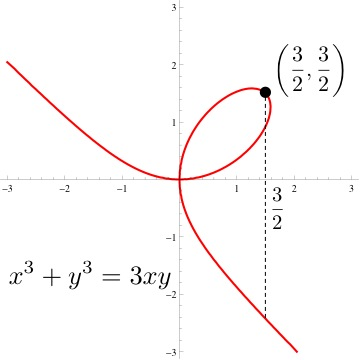
\includegraphics{./images/ch4/x3y33xy.jpg}}
\end{center}

{\bf P186-例29:}设$y=y(x)$是由方程$y^2=x^2-\cos y$所确定的隐函数,求$y''(x)$。

\begin{center}
	\resizebox{!}{6cm}{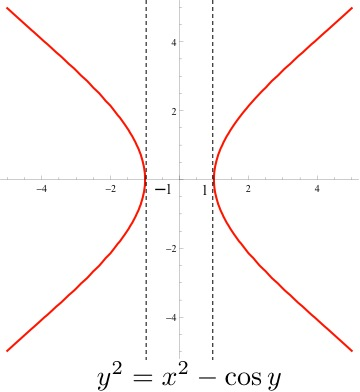
\includegraphics{./images/ch4/y2x2-cosy.jpg}}
\end{center}

{\bf P187-例30:}求函数$y=(x^2+1)\sqrt[3]{(x-2)^2(x^2+x)}$的导数。

\subsection{参数方程求导法则}

设函数$y=y(x)$由参数方程
$$\left\{
\begin{array}{l}
x=\varphi(t)\\
y=\psi(t)
\end{array}
\right.$$
确定, $x=\varphi(t)$可逆, 则
$$y'(x)=\df{\psi'(t)}{\varphi'(t)}$$

$$y''(x)=\df{\psi''(t)\varphi'(t)-\psi'(t)\varphi''(t)}{[\varphi'(t)]^3}$$

{\bf P188-例31:}求抛物线$x=y^2$在$(1,1)$和$(4,-2)$处的切线方程。

{\bf P189-例32:}已知$\left\{\begin{array}{l}x=t-\sin t\\
y=1-\cos t\end{array}\right.$,求$y''(x)$。

\begin{center}
	\resizebox{!}{4cm}{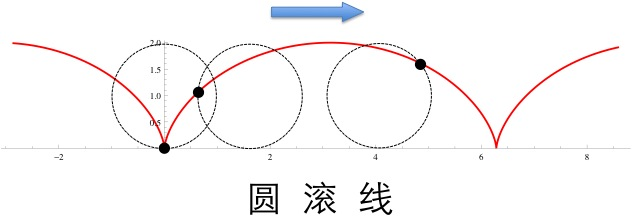
\includegraphics{./images/ch4/sphereRoll.jpg}}
\end{center}

{\bf 例:}设$\left\{\begin{array}{l}x=f\,'(t)\\ y=tf\,'(t)-f(t)
\end{array}\right.$,求$\df{\d^2y}{\d x^2}$,其中$f\,''(x)$存在且不为零。

\section{微分}

\subsection{概念}

{\bf 【局部线性化和“以直代曲”】}

若$f(x)$在$x_0$可导,则
$$f(x)=f(x_0)+f\,'(x_0)(x-x_0)+\circ(x-x_0)\quad(x\to x_0)$$ 
即:{\bf 在$x_0$附近,$f(x)$可以近似地表示为一个线性函数} 
$$f(x)\approx f(x_0)+f\,'(x_0)(x-x_0)$$

\begin{center}
	\resizebox{!}{6cm}{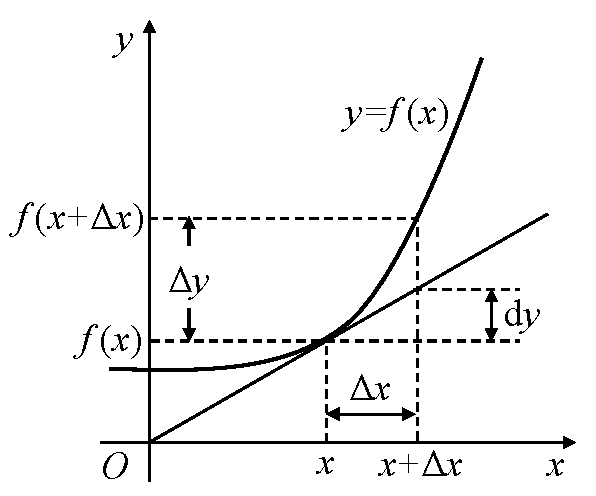
\includegraphics{./images/ch4/dy.pdf}}
\end{center}

{\bf 定义4.3.1:}设$y=f(x)$在$x_0$的某领域内有定义,
若存在与$\Delta x$无关的常数$A$,使得$\Delta y=f(x_0+\Delta x)-f(x_0)$满足
$$\Delta y=A\Delta x+\circ(\Delta x)\;(\Delta x\to 0)$$ 
则称$y=f(x)$在$x_0${\it 可微}, $A\Delta x$称为{\it $y=f(x)$在$x_0$处的微分},
记为 $$\left.\d y\right|_{x=x_0}\quad \mbox{或} \quad
\left.\d f(x)\right|_{x=x_0}$$

{\bf 定理4.3.1:}设$y=f(x)$在$x_0$可微,当且仅当$y=f(x)$在$x_0$可导,且
$$\left.\d y\right|_{x=x_0}=f\,'(x_0)\d x\quad 
\mbox{或} \quad\left.\d f(x)\right|_{x=x_0}=f\,'(x_0)\d x$$

{\bf P196-例3:}设$f(x)=x^3+2x^2-3x+6$,求$\d f(x)$和$\d f(x)|_{x=1}$,
并求其在$(1,6)$处的局部线性化函数$L(x)$。

\subsection{微分的运算法则}

{\bf 定理4.3.2}(四则运算)设$u(x),v(x)$可导,则
\begin{enumerate}[(1)]
  \setlength{\itemindent}{1cm}
  \item $\d (u\pm v)=\d u\pm \d v$
  \item $\d(uv)=v\d u+u\d v$
  \item $\d\df uv=\df{v\d u-u\d v}{v^2}$
\end{enumerate}

{\bf 定理4.3.3}(复合运算)设$y=f(u),u=\varphi(x)$均可微,
则$y=f[\varphi(x)]$可微,
$$\d y=f\,'(u)\d u=f\,'(u)\varphi'(x)\d x$$

{\bf P201-例6:}求函数$y=e^{2x-1}\sin x$的微分。

{\bf P202-例7:}试将下列微分形式表示为某一函数的微分 
\begin{enumerate}[(1)]
  \setlength{\itemindent}{1cm}
  \item $x^2\d x$ 
  \item $e^{2x}\d x$ 
  \item $\cos(5x-1)\d x$ 
  \item $\df{1}{1+2x^2}\d x$
\end{enumerate}

\section{变化率和相关变化率}

{\bf 变化率:}一个变量随另一个变量变化过程中,相对于后者发生变化的速率,或者
{\it 二者的相关变化量的比值}

{\bf 导数:}对于各种变化率的数学抽象

\begin{itemize}
  \setlength{\itemindent}{1cm}
  \item {斜率}:线性函数的函数值关于自变量的变化率 
  \item {速度}:位移关于时间的变化率 
  \item {密度}:质量关于体积的变化率 
  \item {电流强度}:电量关于时间的变化率 
  \item {边际收益}:收益关于投入的变化率 
  \item {\ldots\ldots} 
\end{itemize}

{\bf P209-例7:}有一深度$8$m,上底直径$8$m的圆锥形容器,
以$4$m$^3$/min的速率向其中注水,当容器中水深$5$m时,水面上升的速度是多少?

{\bf P209-例8:}甲乙两船分别向南和向东航行。在初始时刻,甲船恰位于乙船北方
$40$km处,后来在某一时刻测得甲船向南航行了20km,此时速度为15km/h;
乙船向东航行了15km,此时速度为25km/h。问该时刻两船是在相互靠近还是远离,
二者的相对速度是多少?

\begin{shaded}
{\bf 应用题结题的一般步骤}
\begin{enumerate}
  \setlength{\itemindent}{1cm}
  \item {{\bf 画图$^*$:}}画出示意图
  \item {{\bf 确定变量:}}给出各变量的数学符号表示
  \item {{\bf 建立关系:}}根据已知,建立变量关系式
  \item {{\bf 求导:}}对所建立的关系式两边求导
  \item {{\bf 求解:}}整理新的关系式,得出结果
\end{enumerate}
\end{shaded}

\section{不定积分}

\subsection{原函数与不定积分}

{\bf 定义4.5.1:}若在区间$I$上,$f\,'(x)=f(x)$,
则称$F(x)$是{\it $f(x)$在区间$I$上的原函数}。

{\bf 性质:}若$F(x)$是$f(x)$在区间$I$上的原函数,则
\begin{enumerate}
  \setlength{\itemindent}{1cm}
  \item $F(x)+C$也是$f(x)$在区间$I$上的原函数
  \item $f(x)$的任意两个原函数只相差一个常数
\end{enumerate}

{\bf 例:}不定积分表达式的多样形式
\begin{enumerate}[(1)]
  \setlength{\itemindent}{1cm}
  \item $\dint\sin x\cos x\d x=\df12\sin^2x+C$
  \item $\dint\cos x\sin x\d x=\df12\cos^2x+C$
  \item $\dint\df12\sin2x\d x=\cos2x+C$
\end{enumerate}
以上三者都属于同一个函数族,仅相差一个常数!\ps{要想判断它们是否相同,
最可靠的方法还是求导,比较其导函数是否相同}

{\bf 例:}证明:函数$$f(x)=\left\{\begin{array}{ll}
0\;& x\ne 0\\1\;& x=0\end{array}\right.$$在$\mathbb{R}$上不存在原函数

{\bf 注:}{具有第一类间断点的函数都不存在原函数}

{\bf 定理}({\it 原函数的存在性})
若函数$f(x)$在区间$I$上连续,则在$I$上存在原函数。

{\bf 定义4.5.2:}函数$f(x)$在区间$I$上的全体原函数称为{\it $f(x)$在$I$上的不定积分},
记为
$$\int f(x)\d x$$

{\bf 注:}若$F(x)$是$f(x)$在区间$I$上的一个原函数, 则
$${\int f(x)\d x=F(x)+C},$$
其中$C$为任意常数。

{\bf P215-性质4.5.1:}
\begin{enumerate}[(1)]
  \setlength{\itemindent}{1cm}
  \item $\left(\displaystyle\int f(x)\d x\right)'=f(x)$ 
  \item $\d\left[\displaystyle\int f(x)\d x\right]=f(x)\d x$ 
  \item $\dint f\,'(x)\d x =f(x)+C$
  \item $\dint \d f(x)=f(x)+C$
\end{enumerate}

\subsection{基本不定积分公式}

{\it 求不定积分是求导的“逆运算”}
\begin{enumerate} [(1)]
  \setlength{\itemindent}{1cm}
  \item $(C)'=0$\hfill  {$\dint 0\d x=C$} 
  \item $(x^a)'=ax^{a-1}$\hfill  {$\dint x^a\d x=\df{1}{a+1}x^{a+1}+C$}
  \item $(e^x)'=e^x$\hfill  {$\dint e^x\d x=e^x+C$} 
  \item $(a^x)'=a^x\ln a$\hfill  {$\dint a^x\d x=\df{a^x}{\ln a}+C$}
  \item $(\ln x)'=\df 1x$\hfill  {$\dint \df 1x\d x=\ln|x|+C$}
  \item $(\sin x)'=\cos x$\hfill  {$\dint \cos x\d x=\sin x+C$} 
  \item $(\cos x)'=\sin x$\hfill  {$\dint \sin x\d x=-\cos x+C$}
  \item $(\tan x)'=\sec^2 x$\hfill  {$\dint \sec^2 x\d x=\tan x+C$} 
  \item $(\cot x)'=-\csc^2 x$\hfill  {$\dint \csc^2 x\d x=-\cot x+C$}
  \item $(\sec x)'=\sec x\tan x$\hfill $\dint\sec x\tan x\d x=\sec x+C$
  \item $(\csc x)'=-\csc x\cot x$\hfill $\dint\csc x\cot x\d x=-\csc x+C$
  \item $(\arcsin x)'=\df{1}{\sqrt{1-x^2}}$ \hfill  
  {$\dint{\df{1}{\sqrt{1-x^2}}}\d x=\arcsin x+C$} 
  \item $(\arctan x)'=\df{1}{1+x^2}$ \hfill 
  {$\dint \df{1}{1+x^2}\d x=\arctan x+C$}
  \item $(\cosh x)'=\sinh x$ \hfill $\dint\sinh x\d x=\cosh x+C$
  \item $(\sinh x)'=\cosh x$ \hfill $\dint\cosh x\d x=\sinh x+C$
\end{enumerate}

{\bf 注:}$x>0$时,$(\ln x)'=\df 1x$,所以$\dint\df{\d x}x=\ln x+C$,
$x<0$时,$(\ln(-x))'=\df1x$,所以$\dint\df{\d x}x=\ln(-x)+C$

{\bf P217-218:例3-4:}计算不定积分
\begin{enumerate}[(1)]
  \setlength{\itemindent}{1cm}
  \item $\dint x^2\sqrt{x}\d x$ 
  \item $\dint \df{1}{x\sqrt[3]{x}}\d x$ 
  \item $\dint \df{4^x}{9^x}\d x$ 
  \item $\dint 2^x3^{2x}5^{3x}\d x$
\end{enumerate}

\subsection{不定积分的运算法则}

{\bf 性质4.5.2}(线性运算)设函数$f(x),g(x)$的原函数存在,则
$$\int[\alpha f(x)+\beta g(x)]\d x=\alpha\int f(x)\d x+\beta\int g(x)\d x,$$
其中$\alpha,\beta$为任意常数。

{\bf 例:}计算不定积分
\begin{enumerate}[(1)]
  \setlength{\itemindent}{1cm}
  \item $\dint (4x^3-2x^2+5x+3)\d x$
  \item $\dint(1-2x)^2\sqrt x\d x$
  \item $\dint\df{(x-\sqrt x)(1+\sqrt x)}{\sqrt[3]x}\d x$
  \item $\dint\df{\d x}{\sin^2x\cos^2x}$
  \item $\dint(10^x+3\sin x+\sqrt x)\d x$
  \item $\dint\sum\limits_{k=0}^na_kx^k$
\end{enumerate}

{\bf P219-例5-6:}计算不定积分
\begin{enumerate}[(1)]
  \setlength{\itemindent}{1cm}
  \item $\dint (x^2+1)^2\d x$ 
  \item $\dint\df{(x+1)^3}{x^2}\d x$ 
  \item $\dint\df{1-x^2}{x^2(1+x^2)}\d x$
  \item $\dint \df{x^4}{1+x^2}\d x$ 
  \item $\dint\df{1}{1+\cos 2x}\d x$ 
  \item $\dint\tan^2 x\d x$
\end{enumerate}

\section{不定积分的计算}

\subsection{换元法}

{\bf 定理6.3.1}(第一换元法)设$f(u)$具有原函数,$u=\varphi(x)$可导,则
$$\dint f[\varphi(x)]\varphi'(x)\d x=\left[\dint f(u)
\d u\right]_{u=\varphi(x)}$$
{\bf 注:}设$F(x)$是$f(x)$的一个原函数,则
$$\dint f[\varphi(x)]\varphi'(x)\d x=F[\varphi(x)]+C$$

{\bf 例:}计算下列不定积分
\begin{enumerate}[(1)]
  \setlength{\itemindent}{1cm}
  \item $\dint\cos 2x\d x$ 
  \item $\dint\df 1{3+2x}\d x$
  \item $\dint\df{\d x}{x^2-a^2}$
  \item $\dint 2xe^{x^2}\d x$ 
  \item $\dint\df{x^2}{(x+2)^3}\d x$ 
  \item $\dint\df 1{a^2+x^2}\d x$ 
  \item $\dint\df 1{\sqrt{a^2-x^2}}\d x$ 
  \item $\dint \df 1{x(1+2\ln x)}\d x$ 
  \item $\dint\df {e^{3\sqrt x}}{\sqrt x}\d x$ 
  \item $\dint \sin^3x\d x$ 
  \item $\dint \sin^2x\cos^4x\d x$ 
  \item $\dint\sec^6x\d x$ 
  \item $\dint\sec x\d x$
\end{enumerate}

{\bf 注:}另解
$$\dint\sec x\d x=\dint\df{\sec x(\sec x+\tan x)}{(\sec x+\tan x)}\d x
=\dint\df{\d(\sec x+\tan x)}{(\sec x+\tan x)}=
\ln|\sec x+\tan x|+C$$

\begin{shaded}
{\bf 【第一换元法的一些常用技巧】}
\begin{enumerate}
  \setlength{\itemindent}{1cm}
  \item {\bf 分项积分:}积化和差,有理分式分解,\ldots 
  \item {\bf 降低幂次:}倍角公式,万能凑幂公式,\ldots 
    $$\dint f(x^n)x^{n-1}\d x=\df 1n\dint f(x^n)\d x^n$$ 
    $$\dint f(x^n)\df 1x\d x=\df 1n\dint f(x^n)\df{1}{x^n}\d x^n$$ 
  \item {\bf 统一函数:}三角公式,$1=\sin^2x+\cos^2x$,\ldots 
  \item {\bf 巧妙配元:}加一项减一项,\ldots
\end{enumerate}
\end{shaded}

{\bf 定理6.3.2}(第二换元法)设$x=\varphi(t)$可导且可逆,
$f[\varphi(t)]\varphi'(t)$具有原函数,则
$$\dint f(x)\d x=\left[\dint
f[\varphi(t)]\varphi'(t)\d t\right]_{t=\varphi^{-1}(x)}$$

{\bf 例:}计算下列不定积分
\begin{enumerate}[(1)]
  \setlength{\itemindent}{1cm}
  \item $\dint \sqrt{a^2-x^2}\d x$ 
  \item $\dint\df{\d x}{\sqrt{x^2+a^2}}$
  \item $\dint\df{\d x}{(x^2+a^2)^2}$
  \item $\dint\df{\d x}{\sqrt{x^2-a^2}}$ 
  \item $\dint \df{1}{1+\sqrt x}\d x$ 
  \item $\dint\df{\d x}{1+\sqrt[3]{x+2}}$ 
  \item $\dint\df{\sqrt{a^2-x^2}}{x^4}\d x$
\end{enumerate}

\begin{shaded}
{\bf 【第二换元法中的一些特殊变换】}


{\bf 【倒代换】}
当被积函数的分母次数较高,特别是含有无理项时,可尝试令
$$x=\df 1t$$

{\bf 例:}$\dint\df{\d x}{x^3\sqrt{1+x^2}}=-\dint\df{t^2\d t}{\sqrt{1+t^2}}
=-\df{\sqrt{1+x^2}}{2x^2}+\df12\ln\df{1+\sqrt{1+x^2}}{|x|}+C$

{\bf 例:}$\dint\df{\d x}{x^4\sqrt{1+x^2}}=-\dint\df{t^3\d t}{\sqrt{1+x^2}}
=-\df{\sqrt{(1+x^2)^3}}{3x^3}+\sqrt{1+x^2}x+C$

利用公式
$$\dint\df{P_n(x)}y\d x=Q_{n-1}y+\lambda\dint\df{\d x}y$$
(其中$y=\sqrt{qx^2+rx+s}$,$P_n(x),Q_{n-1}(x)$分别为$n$次和$n-1$次多项式)
可将倒代换应用于形如
$$\dint\df{\d x}{x^n\sqrt{ax^2+bx+c}}(n\geq1)$$
的不定积分。

{\bf 例:}$I=\dint\df{x^3\d x}{\sqrt{1+2x-x^2}}$

[hint:] let
$$I=(ax^2+bx+c)\sqrt{1+2x-x^2}+\lambda\dint\df{\d x}{\sqrt{1+2x-x^2}}$$
两边对$x$求导,可解得
$$a=-\df13,\quad b=-\df56,\quad,c=-\df{19}6,\quad\lambda=4$$

{\bf 例:}$I=\dint\df{\d x}{x^n\sqrt{ax^2+bx+c}},(n\geq 1)$

[hint:] let $x=\df 1t$, then
$$I=\dint\df{-t^{n-1}\d t}{\sqrt{a+bt+ct^2}}$$

形如
$$\dint\df{\sqrt{ax^2+bx+c}}{x^n}\d x$$
的积分

{\bf 【Eular代换】}

主要用于处理形如$\dint(R,\sqrt{ax^2+bx+c})$形式的积分,通过Eular代换可以将其化为
有理函数积分,具体代换形式如下:
\begin{enumerate}
  \setlength{\itemindent}{1cm}
  \item 当$a>0$时,令$\sqrt{ax^2+bx+c}\pm\sqrt ax=t$,
  即$x=\df{t^2-c}{b\pm2\sqrt at}$
  \item 当$c>0$时,令$\sqrt{ax^2+bx+c}\pm\sqrt c=tx$,
  即$x=\df{b\pm2\sqrt ct}{t^2-a}$
  \item 当$ax^2+bx+c=0$有两个实根$\alpha$和$\beta$时,
  令$\sqrt{ax^2+bx+c}=t(x-\alpha)$,
  即$x=\df{\alpha\beta-\alpha t^2}{a-t^2}$
\end{enumerate}

{\bf 例:}令$\sqrt{1+x^2}=t-x$,则
$$\dint\df{x^3}{\sqrt{1+x^2}}\d x=\dint\df{(t^2-1)^3}{8t^4}\d t$$

{\bf 例:}令$\sqrt{1+x^2}=xt-1$,则
$$\dint\df{x^3}{\sqrt{1+x^2}}\d x=-16\dint\df{t^3}{(t^2-1)^4}\d t$$
\end{shaded}

\subsection{分部积分法}

$$\dint uv'\d x=uv-\dint u'v\d x$$

{\bf 例:}计算下列不定积分
\begin{enumerate}[(1)]
  \setlength{\itemindent}{1cm}
  \item $\dint x\cos x\d x$ 
  \item $\dint xe^x\d x$ 
  \item $\dint x^2e^x\d x$ 
  \item $\dint\ln x\d x$
  \item $\dint x\ln x\d x$ 
  \item $\dint x\arctan x\d x$ 
  \item $\dint e^x\sin x\d x$
\end{enumerate}

\begin{shaded}
{\bf 【分部积分法处理原则】}
\begin{center}
	{\bf “{反对}不要碰,{三指}动一动”} 
\end{center}
将被积函数视为两个函数之积,按照{\bf{“三指幂对反”}}的次序将其中某一部分函数放到微分符号后面 
\begin{enumerate}
  \item $\sin x,\cos x$ 
  \item $e^x$ 
  \item $x^n$
\end{enumerate}
\end{shaded}

\subsection{有理函数积分}

{\bf 有理函数(有理分式):}$$f(x)=\df{P(x)}{Q(x)}$$
其中$P(x),Q(x)$均为多项式函数 ,若$P(x)$的次数小于$Q(x)$的次数,
称该函数为{\it 真分式} ,否则为{\it 假分式}

{\bf 注:}利用{\it 多项式除法},任意假分式都可以表示成一个多项式与一个真分式的和,例如:
$$\df{2x^4+x^2+3}{x^2+1}=2x^2-1+\df{4}{x^2+1}$$

\begin{shaded}
{\bf 【有理函数分解的一般过程】}

第一步:任意多项式$Q(x)$在实数系内总能分解为一个常数,与形如$(x-a)^n$与$(x^2+px+q)^m$
的诸因式之乘积,其中$a$是$Q(x)$的$n$重根,二次多项式$x^2+px+q$没有实根($p^2-4q<0$),
有共轭复根,且重数均为$m$,故
$$Q(x)=\prod\limits_{i=1}^s(x-a_i)^{\lambda_i}
\prod\limits_{j=1}^t(x^2+p_jx+q_j)^{\mu_j},$$
其中$\lambda_1,\ldots,\lambda_s,\mu_1,\ldots,\mu_t$均为正整数。

第二步:根据代数的分项分式定理,真分式$\df{P(x)}{Q(x)}$可进行如下分解
\begin{eqnarray*}
	\df{P(x)}{Q(x)}&=&\df{A_1}{(x-a_1)^{\lambda_1}}
	+\df{A_2}{(x-a_1)^{\lambda_1-1}}+\ldots
	+\df{A_{\lambda_1}}{x-a_1}+\ldots\\
	&&+\df{B_1}{(x-a_s)^{\lambda_s}}
	+\df{B_2}{(x-a_s)^{\lambda_s-1}}+\ldots
	+\df{B_{\lambda_s}}{x-a_s}+\ldots\\
	&&+\df{M_1x+N_1}{(x^2+p_1x+q_1)^{\mu_1}}
	+\df{M_2x+N_2}{(x^2+p_1x+q_1)^{\mu_1-1}}+\ldots
	+\df{M_{\mu_1}x+N_{\mu_1}}{x^2+p_1x+q_1}+\ldots\\
	&&+\df{U_1x+V_1}{(x^2+p_tx+q_t)^{\mu_t}}
	+\df{U_2x+V_2}{(x^2+p_tx+q_t)^{\mu_t-1}}+\ldots
	+\df{U_{\mu_t}x+V_{\mu_t}}{x^2+p_tx+q_t}
\end{eqnarray*}

第三步:用待定系数法求出以上的所有常数。
\end{shaded}

{\bf 例}(基本的有理函数积分)
\begin{enumerate}[(1)]
  \setlength{\itemindent}{1cm}
  \item $\dint\df A{x-a}\d x=A\ln|x-a|+C$ 
  \item $\dint\df{B\d x}{(x-a)^n}=\df B{(1-n)(x-a)^{n-1}}+C$ 
  \item $\dint\df{Cx+D}{x^2+px+q}\d x=
  \df C2\ln(x^2+px+q)+\df{2D-Cp}{\sqrt{4q-p^2}}
  \arctan\df{2x+p}{\sqrt{4q-p^2}}+C$
  \item $\dint\df{Ex+F}{(x^2+px+q)^m}\d x
  =\df E{2(1-m)(x^2+px+q)^{m-1}}+J_m$,其中:记$u^2=q-p^2/4$,
  $$J_m=\df{y}{2u^2(m-1)(y^2+u^2)^{m-1}}+
  \df{3-2m}{2u^2(1-m)}J_{m-1},$$
  $$J_1=\df1u\arctan\df yu+C$$
\end{enumerate}

{\bf 性质:}
\begin{enumerate}
  \setlength{\itemindent}{1cm}
  \item 设$Q(x)$可分解为两个没有共因式的多项式$Q_1(x),Q_2(x)$的乘积,
  则真分式$\df{P(x)}{Q(x)}$必可分解为
  两个真分式$\df{P_1(x)}{Q_1(x)},\df{P_2(x)}{Q_2(x)}$的和
  \item 任意多项式都可分解为形如$(x^2+px+q)^l$,$(x-a)^k$的多项式的乘积
\end{enumerate}

{\bf 例:}计算下列不定积分
\begin{enumerate}[(1)]
  \setlength{\itemindent}{1cm}
  \item $\dint\df{x+1}{x^2+5x+6}\d x$ 
  \item $\dint\df{x+2}{(2x+1)(x^2+x+1)}\d x$
  \item $\dint\df{x-3}{(x-1)(x^2-1)}\d x$
\end{enumerate}

{\bf 【一些可以化成有理函数的积分】}

{\bf 情形一:}
$$\dint R(\sin x,\cos x)\d x$$
令$t=\tan\df x2$(万能代换),则
$$\sin x=\df{2t}{1+t^2},\quad\cos x=\df{1-t^2}{1+t^2}$$

{\bf 例:}$\dint\df{1+\sin x}{\sin x(1+\cos x)}\d x$

{\bf 情形二:}
$$\dint R(\sin^2x,\cos^2x,\sin x,\cos x)\d x$$
令$t=tan x$

{\bf 例:}$\dint\df{\d x}{a^2\sin^2x+b^2\cos^2x},\;(ab\ne 0)$

{\bf 情形三:}
$$\dint R\left(x,\sqrt[n]{\df{ax+b}{cx+d}}\right),(ad-bc\ne0),$$
令$t=\sqrt[n]{\df{ax+b}{cx+d}}$

{\bf 例:}$\dint\df1x\sqrt{\df{x+2}{x-2}}\d x$

{\bf 例:}$\dint\df{\d x}{(1+x)\sqrt{2+x-x^2}}$

[hint:] let $t=\sqrt{\df{1+x}{2-x}}$, hence $x=\df{2t^2-1}{1+t^2}$
$$\dint\df{\d x}{(1+x)\sqrt{2+x-x^2}}=\dint\df2{3t^2}\d t$$

{\bf 情形四:}
$$\dint R(x,\sqrt{ax^2+bx+c})\d x,\;(a>0,b^2-4ac\ne0)$$
令$u=x+\df b{2a},k^2=\left|\df{4ac-b^2}{4a^2}\right|$,则$ax^2+bx+c$
必为如下三种情形之一
$$|a(u^2+k^2)|,\quad a|u^2-k^2|,\quad a|k^2-u^2|,$$
从而上述无理根式的积分可化为下列三种形式之一
$$\dint R(u,\sqrt{u^2\pm k^2})\d u,\quad\dint R(u,\sqrt{k^2-u^2})\d u,$$
分别令$u=k\tan t,u=k\sec t,u=k\sin t$即可。

{\bf 例:}$\dint\df{\d x}{x\sqrt{x^2-2x-3}}=\df2{\sqrt3}
\arctan\df{\sqrt{x^2-2x-3}}{\sqrt3(x+1)}+C$

[hint:]let $\sqrt{x^2-2x-3}=x-t$, then $I=\df2{\sqrt3}\arctan
\df{\sqrt{x^2-2x-3}-x}{\sqrt3}+C$

{\bf 注:}$\arctan\df{\sqrt{x^2-2x-3}}{\sqrt3(x+1)}-\df{\pi}3=\arctan
\df{\sqrt{x^2-2x-3}-x}{\sqrt3}$,若令$\sqrt{x^2-2x-3}=x+t$,会有类似的效果

{\bf 例}(一些可以化为有理函数的积分)
\begin{enumerate}[(1)]
  \setlength{\itemindent}{1cm}
  \item $\dint\df{1+\sin x}{\sin x(1+\cos x)}\d x$ 
  \item $\dint\df{\sqrt{x-1}}{x}\d x$ 
  \item $\dint\df{\d x}{1+\sqrt[3]{x+2}}$ 
  \item $\dint\df{\d x}{(1+\sqrt[3]{x})\sqrt x}$ 
  \item $\dint\df 1x\sqrt{\df{1+x}{x}}\d x$
\end{enumerate}

{\bf 例:}计算下列不定积分
\begin{enumerate}
  \item $\dint\df{x^2+\sin^2x}{x^2+1}\sec^2x\d x$
  \item $\dint\df 1{(x^2+1)\sqrt{1-x^2}}\d x$
  \item $\dint\df{3\cos x-4\sin x}{\cos x+2\sin x}\d x$
\end{enumerate}

\newpage

\section*{课后作业}

\begin{itemize}
  \item 习题4.1:6,7,8,9,10
  \item 证明过曲线$\sqrt x+\sqrt y=\sqrt a$上任一点$(x_0,y_0)$的切线在两坐标轴上
		的截距之和为常数。
  \item 习题4.2:1,4,6,11,12,10,11,14,15,18,20
  \item 求函数$y=\df{1}{x^2-3x-4}$的$n$阶导函数。
  \item 习题4.3:3,4,8,11
  \item 习题4.4:6,9,12,14,15,17
  \item 习题4.5:1,4,5,6
  \item 习题6.3:4-6
\end{itemize}

{\bf 【课堂练习与思考题】}

\begin{itemize}
  \item 习题4.1:12,13,14,15,16
  \item 习题4.2:5,8,9,16,17,19,22-24
  \item 习题4.3:2,9,10,12-14
  \item 习题4.4:16,17,19
  \item 习题4.5:7-12
\end{itemize}

\end{document}
